\documentclass[11pt]{article}
\usepackage[margin=1in]{geometry}
\usepackage{setspace}
\singlespacing
\usepackage{amsmath,amssymb,amsthm,mathtools}
\usepackage[T1]{fontenc}
\usepackage[utf8]{inputenc}
\usepackage{newtxtext,newtxmath}
\usepackage{booktabs}
\usepackage{tabularx}
\usepackage{array}
\usepackage{tikz}
\usetikzlibrary{arrows.meta,positioning}
\usepackage[ruled]{algorithm2e}
\usepackage{listings}
\usepackage{xcolor}
\definecolor{codegreen}{rgb}{0,0.6,0}
\definecolor{codegray}{rgb}{0.5,0.5,0.5}
\definecolor{codepurple}{rgb}{0.58,0,0.82}
\definecolor{codeblue}{rgb}{0.13,0.29,0.53}
\lstdefinestyle{mystyle}{
commentstyle=\color{codegreen},
keywordstyle=\color{codeblue}\bfseries,
numberstyle=\tiny\color{codegray},
stringstyle=\color{codepurple},
basicstyle=\ttfamily\scriptsize,
breaklines=true,
keepspaces=true,
numbers=left,
numbersep=5pt,
showspaces=false,
showstringspaces=false,
showtabs=false,
tabsize=2,
frame=single,
xleftmargin=12pt,
framexleftmargin=12pt,
captionpos=b
}
\lstset{style=mystyle}
\DeclareMathOperator{\argTopK}{argTopK}
\DeclareMathOperator{\softmax}{softmax}
\theoremstyle{plain}
\newtheorem{theorem}{Theorem}
\newtheorem{corollary}{Corollary}
\newtheorem{lemma}{Lemma}
\newtheorem{proposition}{Proposition}
\theoremstyle{definition}
\newtheorem{definition}{Definition}
\theoremstyle{remark}
\newtheorem{remark}{Remark}
\usepackage{hyperref}
\hypersetup{
colorlinks=true,
linkcolor=blue!70!black,
citecolor=red!70!black,
urlcolor=blue!70!black,
pdftitle={Page-EntroKV: A formal framework for hardware-aligned, entropy-weighted KV-cache eviction under grouped-query attention},
pdfauthor={Inbasekaran S., Naveen Reddie, Sobin C C, Vinod P}
}
\usepackage[capitalize,nameinlink]{cleveref}
\crefname{figure}{Fig.}{Figs.}
\crefname{table}{Table}{Tables}
\crefname{equation}{Eq.}{Eqs.}
\crefname{section}{Section}{Sections}
\crefname{algorithm}{Algorithm}{Algorithms}
\newcommand{\method}{Page-EntroKV}
\newcommand{\HQ}{H_{Q}}
\newcommand{\HKV}{H_{\mathrm{KV}}}
\newcommand{\Dmodel}{D_{\mathrm{model}}}
\newcommand{\Dhead}{D_{\mathrm{head}}}
\newcommand{\Bbatch}{B_{\mathrm{batch}}}
\newcommand{\Nblk}{N_{\mathrm{blocks}}}
\newcommand{\Attn}[2]{\mathbf{A}_{#1,#2}}
\newcommand{\AttnPool}[2]{\mathbf{A}^{\mathrm{pooled}}_{#1,#2}}
\newcommand{\AttnMean}[2]{\mathbf{A}^{\mathrm{mean}}_{#1,#2}}
\newcommand{\Renyi}[2]{\mathcal{H}_{#1}\!\left(#2\right)}
\newcommand{\Collision}[1]{\mathcal{H}_{2}\!\left(#1\right)}
\newcommand{\CollisionSink}[1]{\mathcal{H}^{\mathrm{sink}}_{2}\!\left(#1\right)}
\newcommand{\UOR}{\mathrm{UOR}}
\newcommand{\Group}[1]{\mathrm{Group}(#1)}
\newcommand{\PageSet}{\mathcal{P}}
\newcommand{\RetSet}[2]{\mathcal{K}_{#1,#2}}
\newcommand{\TokSet}[1]{\mathcal{K}_{l,#1}}
\newcommand{\PageImp}[3]{I_{#1,#2}(P_{#3})}
\newcommand{\Ssink}{S_{\mathrm{sink}}}
\newcommand{\GB}{\,\text{GB}}
\newcommand{\TBs}{\,\text{TB/s}}
\newcommand{\TFLOPs}{\,\text{TFLOP/s}}
\tikzset{
flow/.style={draw, rounded corners=3pt, fill=blue!6, text width=0.92\textwidth, inner sep=6pt, align=left, font=\small},
qbox/.style={draw, fill=blue!8, minimum width=22mm, minimum height=9mm, align=center, rounded corners=2pt, font=\small},
pbox/.style={draw, fill=orange!10, text width=0.88\textwidth, inner sep=6pt, align=center, rounded corners=2pt, font=\small},
arr/.style={-{Latex[length=2mm, width=1.4mm]}}
}
\title{Page-EntroKV: A formal framework for hardware-aligned, entropy-weighted KV-cache eviction under grouped-query attention}
\author{Inbasekaran S.\thanks{Corresponding author. SRM Institute of Science and Technology. \texttt{inba.research.turing.labs@gmail.com}} \and Naveen Reddie \and Sobin C C \and Vinod P}
\date{}
\begin{document}
\maketitle
\begin{abstract}
Auto-regressive large language models at long context are bottlenecked by the key--value (KV) cache: caches grow linearly with context length, and every decoded token streams the entire cache through the memory system. Existing dynamic eviction policies score token importance per query head and select tokens independently. Under grouped-query attention (GQA), sibling query heads share one physical KV buffer, so independent per-head selections force a serving engine to retain the union of divergent token sets---by up to the group ratio $r$---while arithmetic mean pooling dilutes the specialized retrieval heads that carry factual recall. We present \textbf{Page-EntroKV}, a formal framework for hardware-aligned KV-cache eviction that replaces head-level selection with entropy-weighted pooling at the physical GQA group level---computed with sink-isolated entropy so that attention-sink heads cannot masquerade as retrieval heads---projects importance onto the discrete PagedAttention page frames that engines actually allocate, and executes eviction exactly at the hardware tuple $(l, g, P_b)$. We formalize the union overhead ratio and intra-group disagreement and prove that they are linked by an exact analytic identity for two-head groups and by two-sided bounds at every group ratio. We prove strict budget preservation for group-level pooling and a finite-context needle-retention bound that arithmetic-mean pooling provably violates; we characterize the temperature limits of the entropy-weighted family; and we give exact per-layer cross-group page accounting. The framework includes a reference implementation of the decision procedure and an instrumented harness for the structural measurements the theory motivates. Its guarantees are architecture-level and invariant to model scale. Pilot measurements in this version are limited to the logs in \cref{sec:results}: $N=180$ structural groups at consensus with $\UOR=1.0$, 9-run needle recall at 958--1990 tokens with pooled-selection retention where mean pooling records 0.0, $B=16$ page-fill with active mass in all slots, and 4 completed LongBench tasks with 11 harness non-completions excluded. Larger-model, long-context and serving evaluation remain future work.
\end{abstract}
\noindent\textit{Keywords:} Grouped-Query Attention \sep PagedAttention \sep KV-cache compression \sep Attention entropy \sep Inference serving \sep Formal analysis
\section{Introduction}
\label{sec:introduction}
Long-context large language models (LLMs) are now deployed for multi-turn agentic workflows, repository-scale code synthesis, and multi-document legal discovery~\cite{bai2023longbench,hsieh2024ruler,meta2024llama3}. Context windows have grown to match, but long-context use remains fragile: reliability degrades with input position~\cite{liu2023lost}. At context lengths of 32k to 128k$^{+}$ tokens, decoding hits a hardware boundary: every decoded token streams the entire key--value (KV) cache from GPU high-bandwidth memory (HBM) into on-chip SRAM, so the decode phase is strictly memory-bound and its cost grows linearly with context length~\cite{pope2022scaling,kwon2023vllm}. At practical batch sizes the KV cache alone can occupy most of the accelerator's memory, capping concurrency and decoding throughput.

Production architectures respond by sharing KV buffers across query heads. Grouped-query attention (GQA)~\cite{ainslie2023gqa}---adopted by Llama-3.1, Qwen-2.5, and Mistral~\cite{meta2024llama3,qwen2024qwen25,jiang2023mistral}---partitions $\HQ$ logical query heads into $\HKV$ physical KV groups, shrinking the cache by the ratio $r=\HQ/\HKV$. In serving runtimes such as vLLM~\cite{kwon2023vllm}, these groups are materialized as block-partitioned tensors of shape $[\Nblk,\ \HKV,\ B,\ \Dhead]$: the sharing is the memory layout itself, not an implementation detail.

This physical layout breaks a core assumption behind prevailing eviction heuristics. Policies such as H2O~\cite{zhang2023h2o}, SnapKV~\cite{li2024snapkv}, and Scissorhands~\cite{liu2023scissorhands} compute token importance per query head and select top-$k$ sets independently. Sibling heads in a GQA group share one physical buffer, so the engine must store the \emph{union} of their selections---up to $r\times$ the intended budget. We formalize this penalty as the \emph{union overhead ratio} (UOR) and connect it exactly to measurable intra-group disagreement (\cref{prop:uorjaccard}). Arithmetic mean pooling fails from the other direction: it dilutes specialized retrieval heads~\cite{wu2024retrievalheads}, averaging a needle token attended to with mass $1-\epsilon$ by one head down to $(1-\epsilon)/r$, below eviction thresholds.

\method{} follows three design principles, each chosen against a specific alternative. Pooling at the physical-group level rather than the head level preserves GQA's memory sharing and keeps the budget exact; head-level selection cannot do both, because the engine stores whatever union the heads produce. Discrete attention entropy---one inner product per head---separates sharp retrieval heads from diffuse background heads, so weighting heads by inverse entropy amplifies exactly the signals that mean pooling destroys; evaluating that entropy on sink-isolated distributions keeps attention-sink heads from being mistaken for retrieval heads. Projecting importance onto discrete PagedAttention page frames \emph{before} eviction, rather than selecting tokens first, makes the compression decision coincide with the hardware allocation tuple $(l, g, P_b)$ and eliminates internal fragmentation and cache-unrolling overhead. \Cref{fig:pipeline_overview} shows the resulting architecture.

The contributions of this paper are formal, algorithmic, and implementational:
\begin{itemize}
\item \textbf{Architectural formulation.} We formalize the GQA structural constraint in dynamic KV-cache eviction through two metrics---the union overhead ratio and intra-group disagreement---linked by an exact identity for two-head groups and sandwiched two-sidedly at every ratio (\cref{sec:background}).
\item \textbf{Algorithmic design.} We design entropy-weighted group pooling around discrete sink-isolated R\'enyi-2 attention entropy, together with a page-frame mapping that evicts exactly at the $(l, g, P_b)$ tuple (\cref{sec:methodology}).
\item \textbf{Theoretical guarantees.} We prove strict budget preservation ($\UOR \equiv 1$), a finite-context needle-retention bound under head specialization with sink isolation, the temperature degeneracies of the pooling family, and page-level union accounting (\cref{sec:theory}).
\item \textbf{Reference implementation.} We provide a complete PyTorch reference implementation of the decision procedure and an instrumented harness for the structural quantities the theory defines (\cref{app:implementation}).
\end{itemize}
This is a theory paper with a pilot measurement tier. The full empirical study---accuracy under compression across model families, serving-level throughput, and population-level structural measurements---remains future work: \cref{sec:protocol} gives the pre-registered design and pilot governance, \cref{sec:results} reports only what the supplied pilot logs contain, and \cref{sec:discussion} separates claims that hold by construction from pilot observations and pending measurements.

The remainder of this paper is organized as follows. \Cref{sec:related} reviews related work. \Cref{sec:background} formalizes the problem and its structural metrics. \Cref{sec:methodology} presents the \method{} design. \Cref{sec:theory} develops the theoretical analysis. \Cref{sec:protocol} pre-registers the evaluation protocol. \Cref{sec:discussion} delimits scope and limitations, and \cref{sec:conclusion} concludes. \Cref{app:notation} summarizes notation, \cref{app:verification} tabulates the guarantee-to-impact mapping, and \cref{app:implementation} gives the reference implementation.
\begin{figure}[t]
\centering
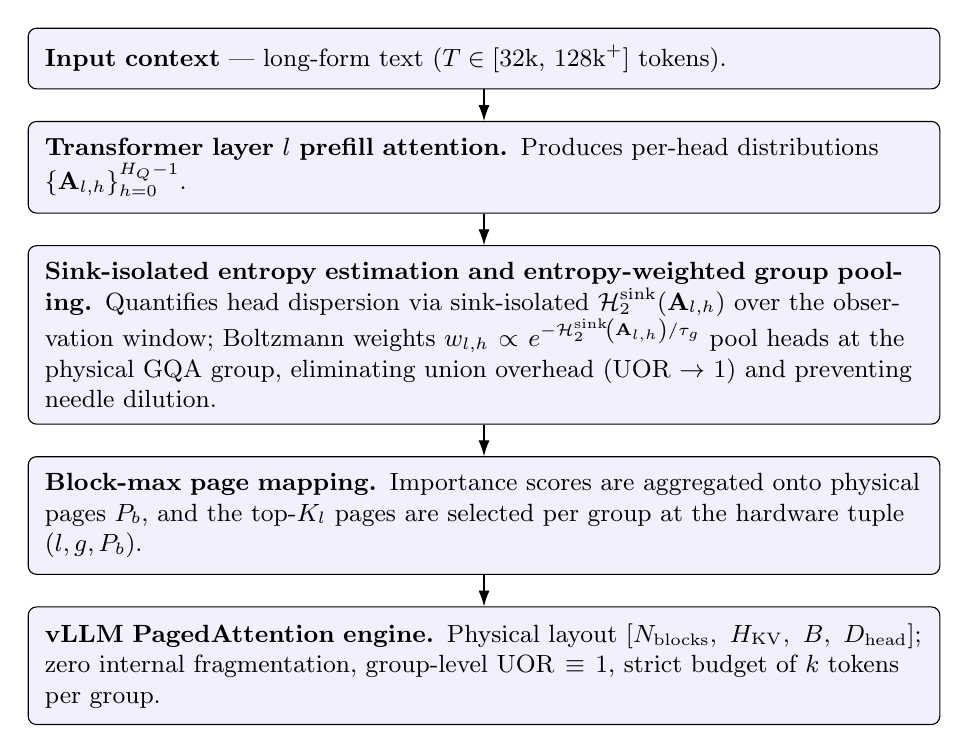
\begin{tikzpicture}[font=\small, node distance=4mm]
\node[flow] (input) {\textbf{Input context} --- long-form text ($T \in [32\text{k},\,128\text{k}^{+}]$ tokens).};
\node[flow, below=of input] (attn) {\textbf{Transformer layer $l$ prefill attention.} Produces per-head distributions $\{\Attn{l}{h}\}_{h=0}^{\HQ-1}$.};
\node[flow, below=of attn] (pool) {\textbf{Sink-isolated entropy estimation and entropy-weighted group pooling.} Quantifies head dispersion via sink-isolated $\CollisionSink{\Attn{l}{h}}$ over the observation window; Boltzmann weights $w_{l,h} \propto e^{-\CollisionSink{\Attn{l}{h}}/\tau_g}$ pool heads at the physical GQA group, eliminating union overhead ($\UOR \to 1$) and preventing needle dilution.};
\node[flow, below=of pool] (page) {\textbf{Block-max page mapping.} Importance scores are aggregated onto physical pages $P_b$, and the top-$K_l$ pages are selected per group at the hardware tuple $(l, g, P_b)$.};
\node[flow, below=of page] (vllm) {\textbf{vLLM PagedAttention engine.} Physical layout $[\Nblk,\ \HKV,\ B,\ \Dhead]$; zero internal fragmentation, group-level $\UOR \equiv 1$, strict budget of $k$ tokens per group.};
\foreach \a/\b in {input/attn, attn/pool, pool/page, page/vllm}
\draw[arr] (\a.south) -- (\b.north);
\end{tikzpicture}
\caption{\method{} pipeline overview. Sink-isolated entropy-weighted pooling at the physical GQA group level, followed by block-max mapping onto PagedAttention page frames, aligns the eviction decision with the engine's physical memory layout.}
\label{fig:pipeline_overview}
\end{figure}
\section{Related work}
\label{sec:related}
\subsection{Attention efficiency and architectural evolution}
Multi-head attention (MHA)~\cite{vaswani2017attention} pairs every query head with private key--value buffers. Multi-query attention (MQA)~\cite{shazeer2019fast} collapses all heads onto a single shared buffer. GQA~\cite{ainslie2023gqa} interpolates between the two, cutting KV memory by the group ratio $r$ at negligible quality cost, and is now standard in production models~\cite{meta2024llama3,qwen2024qwen25,jiang2023mistral}. A separate line compresses KV states into low-rank latent vectors, as in the multi-head latent attention (MLA) of DeepSeek-V2~\cite{deepseek2024deepseekv2}. These works fix the \emph{static} allocation of KV memory. \method{} addresses the complementary \emph{dynamic} problem: deciding at inference time which allocated entries to keep.
\subsection{Inference serving engines}
IO-aware kernel design minimizes HBM traffic. FlashAttention~\cite{dao2022flashattention} tiles attention computation on-chip; FlashAttention-2 adds flash-decoding, improving parallelism for long sequences and decode workloads~\cite{dao2023flashattention2}. On the systems side, vLLM's PagedAttention~\cite{kwon2023vllm} partitions the KV cache into fixed-size blocks managed by a block table and reaches near-zero fragmentation at high concurrency. Orca raises utilization further through iteration-level scheduling and continuous batching~\cite{yu2022orca}. Roofline analyses~\cite{pope2022scaling} establish the memory-bound character of decoding. These engines assume the cache is fully materialized; they define the physical layout to which any compression policy must conform. \method{} treats the page table as a first-class citizen and evicts at exactly the granularity the engine allocates.
\subsection{Dynamic KV-cache eviction}
H2O~\cite{zhang2023h2o} retains tokens with the largest accumulated attention scores. StreamingLLM~\cite{xiao2024streamingllm} preserves attention sinks and a sliding window. Scissorhands~\cite{liu2023scissorhands} exploits the persistence of token importance. SnapKV~\cite{li2024snapkv} compresses the prefill cache using observation windows. PyramidKV~\cite{cai2024pyramidkv} allocates layer-wise budgets following a pyramidal information funnel. Quest~\cite{tang2024quest} performs query-aware sparse selection. FastGen~\cite{ge2024fastgen} selects per-head compression policies from observed attention patterns, adapting the operator while staying at head-level granularity. Ada-KV~\cite{feng2024adakv} works on the budget side of the same GQA structure: it reallocates the per-head eviction budgets within a group adaptively, so the union of head-level selections respects the group budget instead of a uniform per-head quota $k$. Ada-KV decides \emph{how much} each head may keep; it does not change \emph{which} entries survive---selection remains per-head on raw attention scores, with no selection-side guarantee comparable to the needle-retention bound of \cref{thm:needle_preservation}.

All of these methods score importance at the (layer, head) or (layer, token) granularity. Under shared buffers, independent head-level selections inflate memory by up to $r\times$ unless a budget allocator compensates---which is the compensation Ada-KV supplies---and per-head scores cannot be materialized without unrolling the cache. \method{} attacks the inflation at its source: pooling before selection makes the union semantics of GQA harmless by construction, and eviction runs at page granularity.

A concurrent entropy-based method, EntroKV~\cite{entrokv2025}, applies attention entropy at a different decision point. There, Shannon entropy allocates per-layer compression budgets---\emph{how much} each layer keeps---as a plug-and-play front-end, with offline calibration of a mean-entropy statistic $\bar{\mathcal{H}}$. \method{} applies sink-isolated R\'enyi-2 entropy on the selection side---\emph{which} pages survive within each physical group---requires no calibration, and carries the guarantees proved here: group-level $\UOR\equiv 1$ (\cref{thm:memory_guarantee}) and finite-context needle retention (\cref{cor:finite_context_bound}). The two mechanisms sit at different points in the pipeline (budget allocation versus within-group selection); no combination of the two is studied here. \Cref{tab:qualitative} positions \method{} against these families, and against channel-dimension and routing alternatives, along the axes that the GQA layout makes salient.
\begin{table}[t]
\centering\footnotesize
\setlength{\tabcolsep}{3pt}
\caption{Qualitative structural comparison of KV-cache eviction approaches under physically shared GQA buffers. \checkmark\ = supported; $\sim$ = partially; $\times$ = not supported; n/a = not applicable.}
\label{tab:qualitative}
\begin{tabular}{@{}lccccc@{}}
\toprule
Method & Importance & GQA-union & Eviction & Strict budget & Calibration \\
& granularity & aware? & granularity & guarantee? & -free? \\
\midrule
H2O~\cite{zhang2023h2o} & $(l,h,t)$ & $\times$ & token & $\times$ (union $\le r\times$) & \checkmark \\
StreamingLLM~\cite{xiao2024streamingllm} & position & \checkmark\ (uniform) & token & \checkmark\ (static) & \checkmark \\
Scissorhands~\cite{liu2023scissorhands} & $(l,h,t)$ & $\times$ & token & $\times$ & \checkmark \\
SnapKV~\cite{li2024snapkv} & $(l,h)$ & $\times$ & token & $\times$ & \checkmark \\
FastGen~\cite{ge2024fastgen} & per-head policy & $\times$ & token & $\times$ & $\times$ (profiling) \\
PyramidKV~\cite{cai2024pyramidkv} & $(l,h,t)$, layer budget & $\times$ & token & $\sim$ (layer-wise) & \checkmark \\
Quest~\cite{tang2024quest} & query/page & $\times$ & page & $\sim$ (query-dep.) & \checkmark \\
Ada-KV~\cite{feng2024adakv} & $(l,h,t)$, adaptive budget & $\sim$ (budget-side) & token & \checkmark\ (adaptive) & \checkmark \\
EntroKV~\cite{entrokv2025} & $(l,t)$, entropy layer budget & $\times$ & token & $\sim$ (layer-wise) & $\times$ (offline) \\
DuoAttention~\cite{xiao2024duoattention} & head class & $\sim$ (head-level) & head/token & $\times$ & $\times$ (offline) \\
\midrule
\multicolumn{6}{@{}l}{\emph{Channel-dimension and routing alternatives (included for completeness):}}\\
ThinK~\cite{liu2024think} & channel (query-guided) & n/a & channel & $\sim$ (fixed ratio) & \checkmark \\
KIVI~\cite{liu2024kivi} & n/a (2-bit K/V quant.) & n/a & n/a & n/a & \checkmark \\
QuaRot~\cite{ashkboos2024quarot} & n/a (rot.\ + 4-bit) & n/a & n/a & n/a & \checkmark \\
InfLLM~\cite{xiao2024infllm} & query--key block routing & $\sim$ (block-level) & block & $\sim$ & \checkmark\ (training-free) \\
\midrule
\method{} (ours) & $(l,g)$ group & \checkmark & page & \checkmark\ (\cref{thm:memory_guarantee}) & \checkmark\ (runtime entropy) \\
\bottomrule
\end{tabular}
\end{table}
\subsection{Mechanistic head specialization}
Pruning studies showed early that many attention heads are redundant~\cite{michel2019heads,voita2019analyzing}. Retrieval heads carry long-context factuality mechanistically~\cite{wu2024retrievalheads}. DuoAttention~\cite{xiao2024duoattention} statically classifies retrieval versus streaming heads and applies heterogeneous compression---but it classifies offline, at the granularity of the attention computation, and needs a calibration corpus. \method{} weights heads \emph{within} each physical GQA group at runtime, using measured sink-isolated entropy, needs no calibration, and preserves the physical sharing structure of GQA.
\section{Problem formulation and background}
\label{sec:background}
We first fix notation (\cref{tab:notation} in \cref{app:notation}), then characterize the decode-phase memory wall, the physical layout of GQA serving engines, and the structural metrics that quantify why head-independent eviction fails.
\subsection{The decode-phase memory wall}
\label{subsec:roofline}
Decoding runs in two distinct execution regimes. Prefill processes the input prompt via compute-bound matrix--matrix products. Autoregressive decoding emits one token per step: self-attention over historical tokens streams the key--value (KV) cache from high-bandwidth memory (HBM) into on-chip SRAM, reducing the computation to memory-bound matrix--vector products.

Let $\Bbatch$ denote batch size, $L$ transformer layers, $\HQ$ logical query heads, $\HKV$ physical KV heads, $\Dhead$ head dimension, $T$ sequence length, and $b_{\mathrm{el}}$ bytes per element ($b_{\mathrm{el}}=2$ for FP16). Defining the GQA ratio $r \triangleq \HQ/\HKV$, the computational work per decode step is $W_{\mathrm{FLOPs}} = 4\,\Bbatch L\,\HQ\,\Dhead\,T$, while HBM data traffic is $D_{\mathrm{bytes}} = 2\,b_{\mathrm{el}}\,\Bbatch L\,\HKV\,\Dhead\,T + \mathcal{O}(\Dmodel)$. The arithmetic intensity $\mathcal{A}_{\mathrm{decode}}$ is derived as:
\begin{equation}
\mathcal{A}_{\mathrm{decode}}
= \frac{W_{\mathrm{FLOPs}}}{D_{\mathrm{bytes}}}
= \frac{4\,\Bbatch L\,\HQ\,\Dhead\,T}{2\,b_{\mathrm{el}}\,\Bbatch L\,\HKV\,\Dhead\,T + \mathcal{O}(\Dmodel)}
\approx \frac{2r}{b_{\mathrm{el}}},
\label{eq:arithmetic_intensity}
\end{equation}
which yields $\mathcal{A}_{\mathrm{decode}} = 4.0$ FLOP/Byte for 16-bit precision on an $r = 4$ architecture. The hardware ridge point on an NVIDIA H100 SXM5 accelerator ($989.5$\TFLOPs{} dense FP16; $3.35$\TBs{} HBM3 bandwidth) is:
\begin{equation}
I_{\mathrm{ridge}}
= \frac{989.5 \times 10^{12}\ \text{FLOP/s}}{3.35 \times 10^{12}\ \text{Byte/s}}
\approx 295.4\ \text{FLOP/Byte},
\label{eq:ridge_point}
\end{equation}
demonstrating that decoding operates at $< 1.5\%$ of peak compute, strictly memory-bandwidth bound. The total physical KV cache capacity required is:
\begin{equation}
M_{\mathrm{KV}}(T) = 4 \cdot \Bbatch \cdot L \cdot \HKV \cdot \Dhead \cdot T \quad \text{bytes,}
\label{eq:kv_footprint}
\end{equation}
which for Llama-3.1-70B ($L{=}80$, $\HKV{=}8$, $\Dhead{=}128$) with $\Bbatch{=}8$ at $T{=}128\text{k}$ reaches $\approx 343.6$\GB. These figures are architectural constants plus arithmetic; they motivate the compression problem this paper addresses.
\subsection{GQA mechanics and paged memory layout}
\label{subsec:gqa}
Let $\mathbf{X} \in \mathbb{R}^{T \times \Dmodel}$ denote token representations. For query head $h \in \{0, \dots, \HQ-1\}$, mapped to physical group $g(h) = \lfloor h/r \rfloor$, the attention probability vector at a given decode step is:
\begin{equation}
\mathbf{S}_{l,h} = \frac{\mathbf{q}_{l,h}\,\mathbf{K}_{l,g(h)}^{\top}}{\sqrt{\Dhead}}, \qquad \Attn{l,h} = \softmax\!\bigl(\mathbf{S}_{l,h}\bigr) \in \Delta^{T-1},
\label{eq:gqa_attention}
\end{equation}
where $\Delta^{T-1}$ is the probability simplex. MHA corresponds to $r=1$~\cite{vaswani2017attention}, MQA to $\HKV=1$~\cite{shazeer2019fast}, and GQA to $1<\HKV<\HQ$~\cite{ainslie2023gqa}. In vLLM, the physical KV cache is partitioned into non-contiguous page blocks $P_b \in \PageSet$ of fixed capacity $B$ tokens:
\begin{equation}
\mathrm{Shape}\bigl(\mathbf{K}_{\mathrm{physical}}\bigr) = \bigl[\Nblk,\ \HKV,\ B,\ \Dhead\bigr].
\label{eq:paged_layout}
\end{equation}
A logical block table maps $(l,g,\lfloor t/B\rfloor)\mapsto P_b$. Fused CUDA kernels access memory per $(l,g)$ tuple; eviction at sub-page granularity therefore causes internal fragmentation or cache-unrolling overhead.
\subsection{Quantifying the structural breakdown}
\label{subsec:uor}
\begin{definition}[Retention set and union overhead ratio]
\label{def:uor}
Let $\TokSet{h} \triangleq \argTopK_{j \in \{1,\dots,T\}}\bigl(\Attn{l,h,j},\, k\bigr)$ be the set of $k$ token indices selected by head $h$ under per-head budget $k \le T$, with ties broken deterministically by token index so that $\TokSet{h}$ is a single well-defined set. For physical group $g$, the union overhead ratio under head-independent selection is:
\begin{equation}
\UOR(g, k) \triangleq \frac{\bigl|\bigcup_{h \in \Group{g}} \TokSet{h}\bigr|}{k}, \qquad 1.0 \le \UOR(g, k) \le r.
\label{eq:uor_def}
\end{equation}
\end{definition}
\begin{definition}[Intra-group Jaccard disagreement index]
\label{def:jaccard}
The pairwise disagreement between sibling heads $h_i, h_j \in \Group{g}$ is:
\begin{equation}
\mathcal{D}_{\mathrm{Jaccard}}(h_i, h_j) \triangleq 1 - \frac{|\TokSet{h_i} \cap \TokSet{h_j}|}{|\TokSet{h_i} \cup \TokSet{h_j}|}.
\label{eq:jaccard_def}
\end{equation}
\end{definition}
The two metrics are not independent. For a two-head group they determine each other exactly; for general $r$, they sandwich the inflation two-sidedly (\cref{thm:sandwich_bound}). This gives \cref{def:uor,def:jaccard} operational content: measured Jaccard disagreement among sibling heads \emph{implies} a quantifiable memory penalty for any head-independent policy.
\begin{proposition}[Exact UOR--disagreement identity, $r = 2$]
\label{prop:uorjaccard}
Let $r = 2$ and $D = \mathcal{D}_{\mathrm{Jaccard}}(h_1, h_2)$. Then:
\begin{equation}
\UOR(g, k) = \frac{2}{2 - D}.
\label{eq:uor_identity}
\end{equation}
\end{proposition}
\begin{proof}
Let $U = \TokSet{h_1} \cup \TokSet{h_2}$ and $I = \TokSet{h_1} \cap \TokSet{h_2}$. By inclusion--exclusion, $|U| = 2k - |I|$. By definition $D = 1 - |I|/|U|$, so $|I| = (1-D)|U|$. Thus $|U| = 2k - (1-D)|U| \implies (2-D)|U| = 2k$. Dividing by $k$ yields \cref{eq:uor_identity}.
\end{proof}
\begin{corollary}[Elementary Bonferroni certificate]
\label{cor:bonferroni}
Let $J_{ij} = 1 - \mathcal{D}_{\mathrm{Jaccard}}(h_i, h_j)$ and $\bar{J} = \frac{2}{r(r-1)} \sum_{i < j} J_{ij}$. By Bonferroni's inequality:
\begin{equation}
\UOR(g, k) \ge \max\Bigl\{ 1, \; r - r(r-1)\bar{J} \Bigr\}.
\label{eq:bonferroni_bound}
\end{equation}
\cref{eq:bonferroni_bound} certifies a twofold inflation ($\UOR \ge 2$) whenever $\bar{J} \le \frac{r-2}{r(r-1)}$---yielding $\bar{J} \le 1/6$ for $r=4$ and $\bar{J} \le 3/28$ for $r=8$.
\end{corollary}
\begin{proof}
$|\bigcup_h \TokSet{h}| \ge \sum_h |\TokSet{h}| -\sum_{i<j}|\TokSet{h_i}\cap\TokSet{h_j}|$ by Bonferroni, and $|\TokSet{h_i}\cap\TokSet{h_j}| = J_{ij}\,|\TokSet{h_i}\cup\TokSet{h_j}| \le 2kJ_{ij}$. Summing over the $r(r-1)/2$ pairs gives $\sum_{i<j}|\TokSet{h_i}\cap\TokSet{h_j}| \le k\,r(r-1)\bar{J}$, and dividing by $k$ yields the bound; the clamp is $\UOR \ge 1$ from \cref{def:uor}. The threshold follows by solving $r - r(r-1)\bar{J} \ge 2$ for $\bar{J}$.
\end{proof}
\begin{theorem}[GQA inflation sandwich bound]
\label{thm:sandwich_bound}
For general $r \ge 2$, with $J_{ij}$ and $\bar{J} = \frac{2}{r(r-1)}\sum_{i<j}J_{ij}$ as in \cref{cor:bonferroni}, the union overhead ratio is bounded by:
\begin{equation}
\frac{r}{1 + 2(r-1)\dfrac{\bar{J}}{1+\bar{J}}} \;\le\; \UOR(g, k) \;\le\; \min\Biggl(r, \; r - \max_{i < j} \frac{2 J_{ij}}{1 + J_{ij}}\Biggr).
\label{eq:sandwich_bound}
\end{equation}
\end{theorem}
\begin{proof}
\emph{Lower bound.} Let $\mathcal{U} = \bigcup_{i=1}^{r}\TokSet{h_i}$ and define the coverage degree $x_m \triangleq \sum_{i=1}^{r} \mathbf{1}_{\{m \in \TokSet{h_i}\}}$ for $m \in \mathcal{U}$. Exchanging the order of summation and splitting the double sum into diagonal and off-diagonal terms,
\begin{equation}
\sum_{m} x_m = rk, \qquad \sum_{m} x_m^{2} = \sum_{i=1}^{r}\sum_{j=1}^{r} |\TokSet{h_i} \cap \TokSet{h_j}| = rk + 2\sum_{i<j} I_{ij},
\label{eq:coverage_sums}
\end{equation}
where $I_{ij} = |\TokSet{h_i} \cap \TokSet{h_j}|$. Cauchy--Schwarz on $(x_m)$ and the all-ones vector gives $(rk)^{2} \le |\mathcal{U}|\,(rk + 2\sum_{i<j}I_{ij})$, hence $\UOR \ge r^{2}/(r + \tfrac{2}{k}\sum_{i<j}I_{ij})$. From $J_{ij} = I_{ij}/(2k - I_{ij})$ one gets $I_{ij} = 2kJ_{ij}/(1+J_{ij})$, so $\tfrac{2}{k}\sum_{i<j}I_{ij} = 4\sum_{i<j}\frac{J_{ij}}{1+J_{ij}}$. Since $f(x) = \frac{x}{1+x}$ is strictly concave ($f''(x) = -\frac{2}{(1+x)^{3}} < 0$), Jensen's inequality gives $\sum_{i<j} f(J_{ij}) \le \frac{r(r-1)}{2}f(\bar{J})$; substituting this upper bound into the denominator yields the lower bound of \cref{eq:sandwich_bound}. \emph{Upper bound.} For any pair $\{h_a, h_b\}$, $\mathcal{U} = (\TokSet{h_a} \cup \TokSet{h_b}) \cup \bigl(\bigcup_{m \neq a,b}\TokSet{h_m}\bigr)$, so sub-additivity and the map above give $|\mathcal{U}| \le (2k - I_{ab}) + (r-2)k = rk - I_{ab}$, i.e., $\UOR \le r - \frac{2J_{ab}}{1+J_{ab}}$. The pair is arbitrary, so the bound holds with the maximizing pair; the outer $\min(r,\cdot)$ is the natural boundary from \cref{def:uor}.
\end{proof}
\paragraph{Tightness and threshold synchronization.}
The lower bound is tight at both extremes: at $\bar{J}=0$ (pairwise disjoint selections) it evaluates to $r$, the exact worst case, and at $\bar{J}=1$ (identical selections) to $1$, the exact best case. The upper bound is tight at the disjoint extreme; at perfect alignment it evaluates to $r-1$ for $r>2$---mathematically valid, though loose relative to the true limit of $1.0$, because the pairwise profile does not see higher-order overlap structure. Under \cref{thm:sandwich_bound}, twofold inflation ($\UOR \ge 2$) is certified up to $\bar{J} \le \frac{r-2}{3r-2}$---yielding $\bar{J} \le 1/5$ for $r=4$ and $\bar{J} \le 3/11$ for $r=8$---a strictly wider certification range than the Bonferroni threshold of \cref{cor:bonferroni}.

When siblings fully disagree ($\bar{J} \to 0$), they attend to essentially disjoint token sets and $\UOR \to r$: a $4\times$ cache inflation for Llama-3.1-8B ($r=4$) and an $8\times$ inflation for $r=8$ architectures.
\section{The \method{} methodology}
\label{sec:methodology}
\method{} aligns KV-cache eviction with the hardware-physical structure of GQA serving. \Cref{alg:pageentrokv} states the complete decision procedure. \Cref{subsec:entropy} fixes the entropy machinery behind the pooling weights, \cref{subsec:pooling} derives group pooling, page mapping, and eviction, and \cref{subsec:systems} covers integration in vLLM.
\subsection{Sink-isolated discrete R\'enyi attention entropy}
\label{subsec:entropy}
The pooling weights of \method{} come from a discrete entropy family evaluated on sink-isolated attention distributions. This subsection fixes the definitions and the suppression guarantee the rest of the paper relies on.
\begin{definition}[Discrete generalized R\'enyi attention-entropy]
\label{def:renyi}
For $\Attn{l}{h} \in \Delta^{T-1}$ and $\alpha \in (0,1) \cup (1,\infty)$:
\begin{equation}
\Renyi{\alpha}{\Attn{l}{h}} \triangleq \frac{1}{1-\alpha} \ln \Biggl( \sum_{t=1}^T \Attn{l,h}(t)^{\alpha} \Biggr).
\label{eq:renyi_def}
\end{equation}
\end{definition}
Writing $\mathbf{A}\equiv\Attn{l}{h}$ for brevity, taking limits establishes the entropy family:
\begin{align}
\lim_{\alpha \to 1} \Renyi{\alpha}{\mathbf{A}} &= -\sum_{t=1}^T \mathbf{A}(t) \ln \mathbf{A}(t) && \text{(Shannon)}, \label{eq:shannon_limit} \\
\Collision{\mathbf{A}} &= -\ln \sum_{t=1}^T \mathbf{A}(t)^2 = -\ln \|\mathbf{A}\|_2^2 && \text{(collision, } \alpha{=}2\text{)}, \label{eq:collision_entropy} \\
\mathcal{H}_{\infty}(\mathbf{A}) &= -\ln \max_t \mathbf{A}(t) && \text{(min-entropy)}. \label{eq:min_entropy}
\end{align}
We fix $\alpha=2$ for three reasons: collision entropy is a single inner product per head (one warp-level dot product, no per-token logarithms), it is numerically stable in FP16 (\cref{rem:fp16}), and it amplifies attention spikes while suppressing background tail mass.
\begin{definition}[Sink-isolated collision entropy]
\label{def:sinkentropy}
Let $\Ssink$ denote the set of attention-sink tokens, taken as the first $|\Ssink| = 4$ token positions, following the convention of StreamingLLM~\cite{xiao2024streamingllm}. Under the non-degeneracy hypothesis $\sum_{t' \in \Ssink}\Attn{l,h}(t') < 1$ (a head concentrated entirely on $\Ssink$ is handled by the implementation clamp; \cref{rem:fp16}), the sink-isolated attention distribution $\tilde{\mathbf{A}}_{l,h}$ on non-sink positions $t \notin \Ssink$ is:
\begin{equation}
\tilde{\mathbf{A}}_{l,h}(t) \triangleq \frac{\Attn{l,h}(t)}{1 - \sum_{t' \in \Ssink} \Attn{l,h}(t')}, \qquad t \notin \Ssink,
\label{eq:sink_isolated_dist}
\end{equation}
and the sink-isolated collision entropy is $\CollisionSink{\Attn{l}{h}} \triangleq -\ln \|\tilde{\mathbf{A}}_{l,h}\|_2^2$.
\end{definition}
Without isolation, an attention-sink head that concentrates most of its mass on $\Ssink$ has very low raw collision entropy and would receive the same large Boltzmann weight as a genuine retrieval head, misdirecting the pooled mass toward the sink tokens. The next theorem makes the separation quantitative: isolation drives the sink head's weight to zero at a controllable rate while the retrieval head's weight stays bounded away from zero.
\begin{theorem}[Sink head suppression]
\label{thm:sink_suppression}
Let $N = T - |\Ssink|$ and $\tau_g > 0$. Consider two head types: \emph{(i)} a pure sink head concentrating mass $1-\delta$ on $\Ssink$ (with $0<\delta<1$) and a uniform residual over the $N$ non-sink positions; \emph{(ii)} a retrieval head with mass $1-\epsilon'$ at a non-sink needle $t^{*}$ (with $0<\epsilon'<1$) and zero sink mass. Under sink isolation, the sink head has $\|\tilde{\mathbf{A}}\|_2^2 = 1/N$, hence $\CollisionSink{} = \ln N$ exactly, and its Boltzmann factor is:
\begin{equation}
e^{-\CollisionSink{}/\tau_g} = e^{-\ln(N)/\tau_g} = N^{-1/\tau_g} = \frac{1}{(T - |\Ssink|)^{1/\tau_g}} \;\xrightarrow[T \to \infty]{}\; 0,
\label{eq:sink_decay}
\end{equation}
whereas the retrieval head maintains $\CollisionSink{\Attn{l}{h'}} = -2\ln(1-\epsilon') = \mathcal{O}(1)$ and factor $(1-\epsilon')^{2/\tau_g} > 0$: its weight is bounded away from zero for every $T$.
\end{theorem}
\begin{proof}
For the sink head, the residual is uniform: $\tilde{\mathbf{A}}_{l,h}(t) = (\delta/N)/\delta = 1/N$ on all $N$ non-sink positions, so $\|\tilde{\mathbf{A}}\|_2^2 = N \cdot N^{-2} = 1/N$ and $\CollisionSink{} = -\ln(1/N) = \ln N$; its factor is $e^{-\ln N/\tau_g} = N^{-1/\tau_g} \to 0$. For the retrieval head, zero sink mass makes isolation the identity, so $\|\tilde{\mathbf{A}}_{l,h'}\|_2^2 \ge (1-\epsilon')^{2}$ and the factor is at least $e^{2\ln(1-\epsilon')/\tau_g} = (1-\epsilon')^{2/\tau_g}$. For contrast, the \emph{raw} collision entropy of the sink head tends to $-2\ln(1-\delta)$---also $\mathcal{O}(1)$---so raw entropy cannot separate the two types; the separation is created by the isolation step, not by the entropy family alone.
\end{proof}
\begin{definition}[Prefill observation window]
\label{def:obswindow}
The sink-isolated collision entropies used for head weighting are evaluated over the prefill observation window $W_{\mathrm{obs}}$, the final $\min(T, W_{\max})$ tokens of the prompt with $W_{\max}=4096$ (the observation-window convention of SnapKV~\cite{li2024snapkv}):
\begin{equation}
\CollisionSink{\Attn{l}{h}\upharpoonright W_{\mathrm{obs}}} = -\ln \bigl\| \tilde{\mathbf{A}}_{l,h} \upharpoonright W_{\mathrm{obs}} \bigr\|_2^2,
\label{eq:window_entropy}
\end{equation}
where the restriction is renormalized over the window (the normalization constant is part of the configuration and is recorded with it). The entropies---and hence the pooling weights of \cref{eq:boltzmann_weights}---are computed once, at the end of prefill, and remain fixed for the entire auto-regressive generation lifecycle.
\end{definition}
\subsection{Hardware-aligned group pooling and paged mapping}
\label{subsec:pooling}
\begin{figure}[t]
\centering
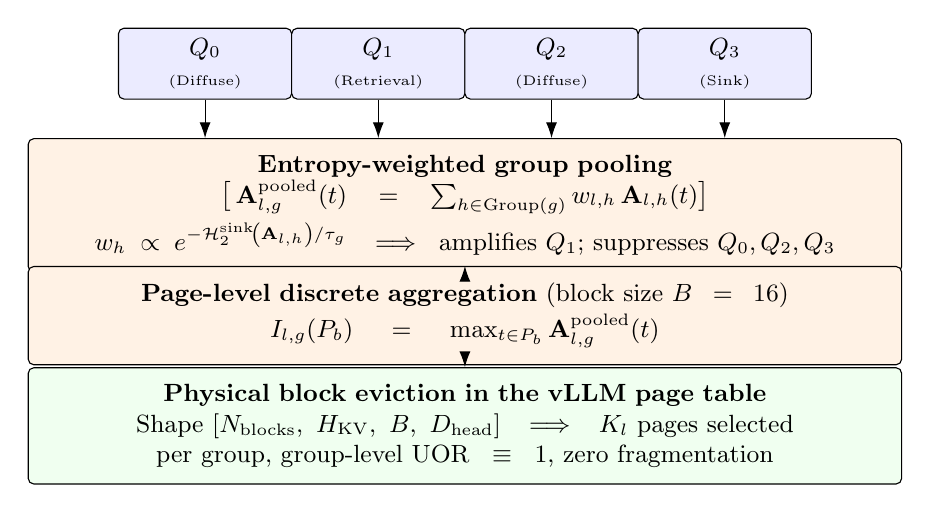
\begin{tikzpicture}[font=\small, node distance=5mm]
\node[qbox] (q0) at (-33mm, 0) {$Q_0$\\{\tiny(Diffuse)}};
\node[qbox] (q1) at (-11mm, 0) {$Q_1$\\{\tiny(Retrieval)}};
\node[qbox] (q2) at (11mm, 0) {$Q_2$\\{\tiny(Diffuse)}};
\node[qbox] (q3) at (33mm, 0) {$Q_3$\\{\tiny(Sink)}};
\node[pbox] (pool) at (0, -18mm) {\textbf{Entropy-weighted group pooling} $\;\bigl[\,\AttnPool{l}{g}(t) = \sum_{h\in\Group{g}}w_{l,h}\,\Attn{l}{h}(t)\bigr]$\\[2pt] $w_h \propto e^{-\CollisionSink{\Attn{l}{h}}/\tau_g} \;\Longrightarrow\;$ amplifies $Q_1$; suppresses $Q_0,Q_2,Q_3$};
\foreach \q in {q0,q1,q2,q3}
\draw[arr] (\q.south) -- (\q.south |- pool.north);
\node[pbox] (page) at (0, -32mm) {\textbf{Page-level discrete aggregation} (block size $B=16$)\\[2pt] $\PageImp{l}{g}{b} = \max_{t\in P_b}\AttnPool{l}{g}(t)$};
\draw[arr] (pool.south) -- (page.north);
\node[pbox, fill=green!6] (vllm) at (0, -46mm) {\textbf{Physical block eviction in the vLLM page table}\\ Shape $[\Nblk,\ \HKV,\ B,\ \Dhead]$ $\;\Longrightarrow\;$ $K_l$ pages selected per group, group-level $\UOR \equiv 1$, zero fragmentation};
\draw[arr] (page.south) -- (vllm.north);
\end{tikzpicture}
\caption{\method{} mechanism for an $r=4$ architecture such as Llama-3.1-8B: entropy-weighted pooling with sink-isolated entropy amplifies the retrieval head $Q_1$, suppresses diffuse heads $Q_0$, $Q_2$, and the attention-sink head $Q_3$, and maps the result onto physical PagedAttention blocks.}
\label{fig:mechanism}
\end{figure}
\paragraph{The union overhead dilemma.}
If selection occurs independently per query head with $\TokSet{h}=\argTopK(\Attn{l,h},k)$, the engine must retain the union $\bigcup_{h\in\Group{g}}\TokSet{h}$, with $\UOR(g,k)\in[1,r]$ as defined in \cref{eq:uor_def}, exactly determined by disagreement at $r=2$ (\cref{prop:uorjaccard}) and sandwiched at every ratio (\cref{thm:sandwich_bound}): an $800\%$ memory expansion for $r=8$ architectures when selections diverge, causing out-of-memory faults.
\paragraph{Needle dilution under arithmetic mean pooling.}
Naive mean pooling assigns
\begin{equation}
\AttnMean{l}{g}(t^{*}) = \frac{1}{r}\!\left[(1-\epsilon)+(r-1)\frac{1}{T}\right] \xrightarrow[T\to\infty]{} \frac{1-\epsilon}{r}.
\label{eq:mean_dilution}
\end{equation}
The needle's pooled mass drops by exactly $1-1/r$---$87.5\%$ for $r=8$, independent of $\epsilon$; for $\epsilon=0.05$ the pooled score is $(1-\epsilon)/8=0.11875$, below common eviction thresholds.
\paragraph{Entropy-weighted group pooling.}
\method{} replaces mean pooling with entropy-weighted group pooling:
\begin{equation}
w_{l,h} = \frac{\exp\bigl(-\CollisionSink{\Attn{l}{h}}/\tau_g\bigr)}{\sum_{j \in \Group{g}} \exp\bigl(-\CollisionSink{\Attn{l}{j}}/\tau_g\bigr)}, \qquad \textstyle\sum_{h \in \Group{g}} w_{l,h} = 1,
\label{eq:boltzmann_weights}
\end{equation}
\begin{equation}
\AttnPool{l}{g}(t) = \sum_{h \in \Group{g}} w_{l,h}\,\Attn{l,h}(t).
\label{eq:pooled_attention}
\end{equation}
Low-entropy retrieval heads receive exponentially larger weights; diffuse streaming heads and attention-sink heads are suppressed, the latter by \cref{def:sinkentropy,thm:sink_suppression}. Pooling runs once per physical KV group---matching how GQA shares memory. The pooled output stays a convex combination of probability vectors, and that property is exactly what the budget guarantee of \cref{thm:memory_guarantee} requires. With $\Ssink=\emptyset$, \cref{eq:boltzmann_weights} reduces to raw collision entropy. The temperature $\tau_g$ interpolates the entire family of group aggregators; we characterize it exactly:
\begin{proposition}[Temperature monotonicity and limits]
\label{prop:temperature_limits}
Let $w_{l,h}(\tau_g)$ be defined by \cref{eq:boltzmann_weights}. \textup{(i)} $w_{l,h}(\tau_g)$ is non-increasing in $\CollisionSink{\Attn{l}{h}}$ (strictly decreasing when the entropies are distinct), for every $\tau_g>0$. \textup{(ii)} $\lim_{\tau_g \to \infty} w_{l,h}(\tau_g) = 1/r$ (arithmetic mean pooling). \textup{(iii)} $\lim_{\tau_g \to 0^+} w_{l,h}(\tau_g)$ is the uniform weight on the set of entropy minimizers---one-hot for a unique minimizer.
\end{proposition}
\begin{proof}
$w$ is a softmax of the scores $-\CollisionSink{\Attn{l}{h}}/\tau_g$, which is strictly increasing in its score; hence $w$ is non-increasing in the entropy (strictly under distinct values). (ii) The entropies are bounded by $\ln T$, so every exponential tends to $1$ and $w \to 1/r$. (iii) Multiplying numerator and denominator by $e^{\mathcal{H}_{\min}/\tau_g}$, every exponent is $\le 0$, equals $0$ exactly at the minimizers, and $e^{-c/\tau_g} \to 0$ for each $c>0$.
\end{proof}
\Cref{prop:temperature_limits} also motivates the failure-mode fallback of \cref{sec:discussion}: when intra-group entropies are indistinguishable, \cref{prop:temperature_limits}~(i) loses its bite, the entropy signal carries no information, and the operator can switch to max-over-heads aggregation without changing the budget guarantee---which depends only on pooling \emph{before} selection (\cref{thm:memory_guarantee}).
\paragraph{Discrete physical block-frame aggregation.}
Token scores are aggregated onto physical page frames $P_b \in \PageSet$ via max-reduction, and the eviction operator selects the top $K_l$ pages at the hardware tuple $(l,g,P_b)$:
\begin{equation}
\PageImp{l}{g}{b} = \max_{t \in P_b} \AttnPool{l}{g}(t), \qquad \RetSet{l}{g} = \mathrm{TopK}\Bigl(\{I_{l,g}(P_b)\}_{P_b \in \PageSet},\ K_l\Bigr).
\label{eq:page_aggregation}
\end{equation}
(Page-level retention sets $\RetSet{l}{g}=\mathcal{K}_{l,g}$ are distinguished from the token-level selection sets $\TokSet{h}$ of \cref{def:uor} by their group subscript.)
\begin{proposition}[Budget initialization and exact conservation]
\label{prop:budget_conservation}
With total budget $\mathcal{B}_{\mathrm{total}}$, the per-layer token budget $\mathcal{B}_l$ and static per-group page quota $K_l$ are:
\begin{equation}
\mathcal{B}_l = \frac{\mathcal{B}_{\mathrm{total}}}{L}, \qquad K_l = \Bigl\lfloor \frac{\mathcal{B}_l}{\HKV \cdot B} \Bigr\rfloor.
\label{eq:page_quotas}
\end{equation}
\textup{(i)} Under the floor quotas alone, exact conservation ($\sum_l \HKV B\,K_l = \mathcal{B}_{\mathrm{total}}$) holds iff $\mathcal{B}_{\mathrm{total}} \equiv 0 \pmod{L\,\HKV\,B}$. \textup{(ii)} With largest-remainder (Hamilton) rounding over the fractional remainders $R_l = \frac{\mathcal{B}_l}{\HKV B} - K_l \in [0,1)$---allocating $+1$ page to the largest-remainder layer-groups---exact conservation holds iff $\HKV\,B$ divides $\mathcal{B}_{\mathrm{total}}$, in which case at most $L-1$ extra page-groups suffice. \textup{(iii)} Otherwise the residual $\mathcal{B}_{\mathrm{total}} \bmod \HKV\,B < \HKV\,B$ tokens---less than one page-group---is unavoidable at page granularity.
\end{proposition}
\begin{proof}
Page allocation is quantized in $\HKV B$ tokens per layer-group, so $\sum_l \HKV B\,K_l$ is always a multiple of $\HKV B$; it equals $\mathcal{B}_{\mathrm{total}}$ iff $\HKV B$ divides $\mathcal{B}_{\mathrm{total}}$, which proves (ii)'s necessity and (iii). For (i): with uniform budgets, $\mathcal{B}_l/(\HKV B) = \mathcal{B}_{\mathrm{total}}/(L\,\HKV B)$, so all $L$ floors sum to $\mathcal{B}_{\mathrm{total}}$ iff the quotient is an integer. For (ii)'s sufficiency: writing $x = \mathcal{B}_{\mathrm{total}}/(\HKV B) \in \mathbb{N}$, the floor sum is $L\lfloor x/L\rfloor$ and the deficit $x - L\lfloor x/L\rfloor \in \{0,\dots,L-1\}$ is distributed as $+1$ allocations to the largest-remainder layers, restoring $\sum_l K_l = x$.
\end{proof}
\paragraph{Page-level retention across groups.}
Because PagedAttention blocks are shared across the $\HKV$ groups of a sequence, per-group retention sets are materialized by the engine as their per-layer union. \Cref{prop:engine_page_accounting} gives the exact accounting.
\begin{proposition}[Engine-level page accounting]
\label{prop:engine_page_accounting}
Let $P^{\mathrm{ret}}_l = \bigcup_g \RetSet{l}{g}$ be the layer page union, where each $\RetSet{l}{g}$ is given by \cref{eq:page_aggregation}. Then, unconditionally:
\begin{equation}
K_l \le \bigl| P^{\mathrm{ret}}_l \bigr| \le \HKV\, K_l.
\label{eq:engine_union_bounds}
\end{equation}
The lower bound is attained iff all groups select identical page sets; the upper bound iff selections are pairwise disjoint.
\end{proposition}
\begin{proof}
By \cref{eq:page_aggregation}, each group retains exactly $K_l$ pages (exact TopK cardinality), so $|\RetSet{l}{g}|=K_l$ for every $g$; the union contains any single member, giving the lower bound. The union of $\HKV$ sets of cardinality $K_l$ each has cardinality at most $\HKV\,K_l$. The equality conditions are immediate.
\end{proof}
The page-union ratio, taken relative to the per-group retention cardinality $|P^{\mathrm{ret}}_l|/K_l$, lies in $[1,\ \HKV]$ and equals one whenever the per-group pooled page profiles coincide. \Cref{prop:engine_page_accounting} states the guarantee at the level where it holds---per layer, across the $\HKV$ groups, on top of the per-group guarantee of \cref{thm:memory_guarantee}---and quantifies the residual overhead exactly. Measuring its typical magnitude across models is part of the protocol in \cref{sec:protocol}.
\subsection{Systems integration in vLLM}
\label{subsec:systems}
\begin{figure}[t]
\centering
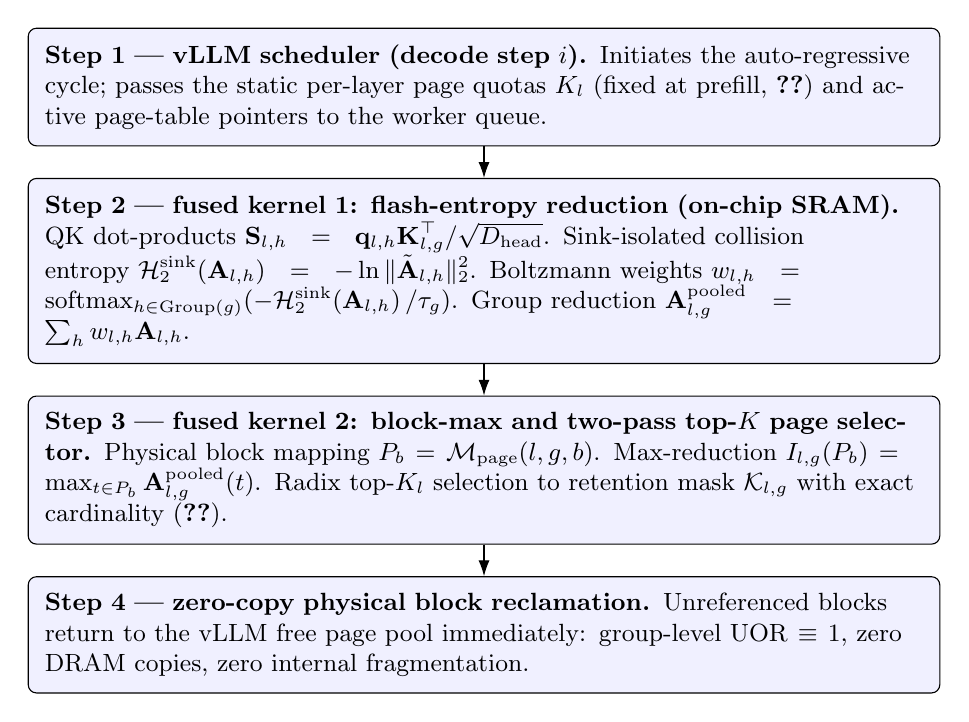
\begin{tikzpicture}[font=\small, node distance=4mm]
\node[flow] (step1) {\textbf{Step 1 --- vLLM scheduler (decode step $i$).} Initiates the auto-regressive cycle; passes the static per-layer page quotas $K_l$ (fixed at prefill, \cref{eq:page_quotas}) and active page-table pointers to the worker queue.};
\node[flow, below=of step1] (step2) {\textbf{Step 2 --- fused kernel 1: flash-entropy reduction (on-chip SRAM).} QK dot-products $\mathbf{S}_{l,h}=\mathbf{q}_{l,h}\mathbf{K}_{l,g}^{\top}/\sqrt{\Dhead}$. Sink-isolated collision entropy $\CollisionSink{\Attn{l}{h}}=-\ln\|\tilde{\mathbf{A}}_{l,h}\|_2^2$. Boltzmann weights $w_{l,h}=\mathrm{softmax}_{h\in\Group{g}}(-\CollisionSink{\Attn{l}{h}}/\tau_g)$. Group reduction $\AttnPool{l}{g}=\sum_h w_{l,h}\Attn{l}{h}$.};
\node[flow, below=of step2] (step3) {\textbf{Step 3 --- fused kernel 2: block-max and two-pass top-$K$ page selector.} Physical block mapping $P_b = \mathcal{M}_{\mathrm{page}}(l,g,b)$. Max-reduction $\PageImp{l}{g}{b}=\max_{t\in P_b}\AttnPool{l}{g}(t)$. Radix top-$K_l$ selection to retention mask $\RetSet{l}{g}$ with exact cardinality (\cref{rem:topk}).};
\node[flow, below=of step3] (step4) {\textbf{Step 4 --- zero-copy physical block reclamation.} Unreferenced blocks return to the vLLM free page pool immediately: group-level $\UOR \equiv 1$, zero DRAM copies, zero internal fragmentation.};
\foreach \a/\b in {step1/step2, step2/step3, step3/step4}
\draw[arr] (\a.south) -- (\b.north);
\end{tikzpicture}
\caption{Hardware-level execution flow of the fused \method{} kernels within the vLLM decoding loop.}
\label{fig:systems_flow}
\end{figure}
\method{} never materializes $\HQ\times T$ intermediate attention matrices in global DRAM. Entropy estimation, Boltzmann weighting, and page reduction are fused into two kernels executing in on-chip SRAM (\cref{fig:systems_flow}). Kernel~1 computes QK dot-products, sink-isolated collision entropies, and Boltzmann weights in FP16 registers, then performs the group reduction in shared memory. Kernel~2 applies the block-table mapping, runs the max-reduction per physical page, and performs two-pass radix top-$K_l$ selection, emitting the retention mask without DRAM materialization. Unreferenced blocks return to the vLLM free-page pool immediately. \Cref{app:implementation} gives the PyTorch reference implementation.
\begin{algorithm}[t]
\DontPrintSemicolon
\footnotesize
\KwIn{$\{\Attn{l}{h}\}_{h=0}^{\HQ-1}$ per layer $l$; $\mathcal{B}_{\mathrm{total}}$; $B$; $\tau_g$; $\Ssink$}
\KwOut{retention masks $\RetSet{l}{g}$ for all $(l,g)$}
$\mathcal{B}_l \leftarrow \mathcal{B}_{\mathrm{total}}/L$;\quad $K_l \leftarrow \lfloor \mathcal{B}_l/(\HKV\cdot B)\rfloor$ \tcp*{Eq.\ \ref{eq:page_quotas}}
\For{$l \leftarrow 1$ \KwTo $L$}{
\For{$g \leftarrow 0$ \KwTo $\HKV-1$}{
$\CollisionSink{\Attn{l}{h}} \leftarrow -\ln\|\tilde{\mathbf{A}}_{l,h}\|_2^2$ over $W_{\mathrm{obs}}$,\; $h\in\Group{g}$\;
$w_{l,h} \leftarrow \mathrm{softmax}_{h\in\Group{g}}(-\CollisionSink{\Attn{l}{h}}/\tau_g)$\;
$\AttnPool{l}{g} \leftarrow \sum_{h\in\Group{g}} w_{l,h}\Attn{l}{h}$\;
$\PageImp{l}{g}{b} \leftarrow \max_{t\in P_b}\AttnPool{l}{g}(t)$\;
$\RetSet{l}{g} \leftarrow \mathrm{TopK}(\{\PageImp{l}{g}{b}\}_{P_b\in\PageSet},\,K_l)$\;
}
}
evict every $P_b \notin \bigl(\bigcup_g \RetSet{l}{g}\bigr)$ per layer; free blocks to the vLLM pool\;
\caption{The \method{} decision procedure.}
\label{alg:pageentrokv}
\end{algorithm}
\section{Theoretical analysis}
\label{sec:theory}
Two guarantees carry the framework. The memory bound of \cref{thm:memory_guarantee} holds by construction, for any attention pattern; the needle-retention result of \cref{thm:needle_preservation} holds under explicit head-specialization assumptions. The remaining results give the finite-context form, a concrete instantiation, and the on-chip cost of the design.
\begin{theorem}[Strict physical memory bounds and union elimination]
\label{thm:memory_guarantee}
Under head-independent top-$k$ eviction, physical memory consumption satisfies:
\begin{equation}
k \le M_{\mathrm{indep}} \le \min(r \cdot k,\, T).
\label{eq:indep_bounds}
\end{equation}
Under \method{} group-level pooling, $M_{\mathrm{pooled}} \equiv k$, guaranteeing group-level $\UOR(g, k) \equiv 1.0$.
\end{theorem}
\begin{proof}
Under head-independent selection, each $h\in\Group{g}$ selects $\TokSet{h}=\mathrm{TopK}(\Attn{l,h},k)$ with $|\TokSet{h}|=k$. Because the KV buffer is physically shared, the engine allocates $\mathcal{K}^{\mathrm{union}}_{g}=\bigcup_{h\in\Group{g}}\TokSet{h}$. Lower bound: the union contains any member set, so $M_{\mathrm{indep}}\ge k$. Upper bound: sub-additivity gives $M_{\mathrm{indep}}\le\sum_h|\TokSet{h}|=rk$, and trivially $M_{\mathrm{indep}}\le T$; hence \cref{eq:indep_bounds}. In \method{}, pooling occurs prior to selection: because $w_{l,h} \ge 0$ and $\sum_h w_{l,h} = 1$, $\AttnPool{l}{g} = \sum_h w_{l,h} \Attn{l,h}$ is a convex combination of probability vectors, so $\AttnPool{l}{g} \in \Delta^{T-1}$ is itself a valid probability vector. Selection is performed on this single pooled vector: $S^{\mathrm{pooled}}_{l,g} = \mathrm{TopK}(\AttnPool{l}{g}, k)$. By the exact cardinality property of TopK on a single vector---with deterministic tie-breaking---$|S^{\mathrm{pooled}}_{l,g}| \equiv k$ under all attention configurations, guaranteeing $\UOR(g,k) = k/k \equiv 1.0$. The union semantics that produce the upper regime of \cref{eq:indep_bounds} are eliminated by construction, for every overlap profile of \cref{subsec:uor}.
\end{proof}
\begin{theorem}[Needle retrieval preservation under head specialization]
\label{thm:needle_preservation}
Suppose $\Group{g}$ contains exactly one retrieval head $h^{*}$ with $\Attn{l,h^{*}}(t^{*})=1-\epsilon$ at a non-sink position $t^{*}\notin\Ssink$, $\epsilon\in(0,\tfrac{1}{2})$, and sink-isolated collision entropy $\CollisionSink{\Attn{l}{h^{*}}}\le\eta_{\mathrm{ret}}$. Suppose each of the $r-1$ sibling heads has near-maximal sink-isolated entropy: there exist constants $c_j\ge 0$, independent of $T$, with
\begin{equation}\label{eq:sibling}
\CollisionSink{\Attn{l}{j}} \;\ge\; \ln\!\bigl(T-|\Ssink|\bigr)-c_j \qquad (j\neq h^{*}).
\end{equation}
Both canonical background cases satisfy \cref{eq:sibling} with $c_j=0$: uniformly diffuse heads, and attention-sink heads whose residual mass is spread (\cref{thm:sink_suppression}); the constant $c_j$ permits mildly concentrated residuals. Then: \textup{(i)} Under arithmetic mean pooling, $\AttnMean{l}{g}(t^{*})\to(1-\epsilon)/r$ as $T\to\infty$. \textup{(ii)} Under entropy-weighted pooling with sink-isolated entropies and temperature $\tau_g>0$: $\lim_{T\to\infty}\AttnPool{l}{g}(t^{*})=1-\epsilon$.
\end{theorem}
\begin{proof}
Write $p_j=\sum_{t'\in\Ssink}\Attn{l,j}(t')$ for the sink mass of sibling $j$, so that $\Attn{l,j}(t)=(1-p_j)\,\tilde{\mathbf{A}}_{l,j}(t)$ for non-sink $t$; in particular $0\le\Attn{l,j}(t^{*})\le\tilde{\mathbf{A}}_{l,j}(t^{*})$.

Part (i): arithmetic mean collapse. For each sibling, \cref{eq:sibling} gives $\|\tilde{\mathbf{A}}_{l,j}\|_2^2=e^{-\CollisionSink{\Attn{l}{j}}}\le e^{c_j}(T-|\Ssink|)^{-1}$, hence $\tilde{\mathbf{A}}_{l,j}(t^{*})\le e^{c_j/2}(T-|\Ssink|)^{-1/2}$ and $\Attn{l,j}(t^{*})\le e^{c_j/2}(T-|\Ssink|)^{-1/2}\to 0$. Therefore
\begin{equation}
\AttnMean{l}{g}(t^{*}) = \frac{1}{r}\Bigl[(1-\epsilon)+\sum_{j\neq h^{*}} \Attn{l,j}(t^{*})\Bigr] \xrightarrow{T\to\infty} \frac{1-\epsilon}{r},
\end{equation}
which equals $(1-\epsilon)/8$ for $r=8$; at the representative $\epsilon=0.05$ this is $0.11875$.

Part (ii): entropy-weighted pooling asymptotics. Let $u_h=\exp(-\CollisionSink{\Attn{l}{h}}/\tau_g)$. The retrieval head satisfies $u_{h^{*}}\ge\exp(-\eta_{\mathrm{ret}}/\tau_g)=C_{\mathrm{ret}}>0$. Each sibling satisfies, by \cref{eq:sibling}, $u_j\le e^{c_j/\tau_g}(T-|\Ssink|)^{-1/\tau_g}$; collecting these, $D(T)\triangleq\sum_{j\neq h^{*}}e^{c_j/\tau_g}(T-|\Ssink|)^{-1/\tau_g}\to 0$ for any fixed $c_j$ and $\tau_g>0$. Hence $w_{l,h^{*}}\ge\frac{C_{\mathrm{ret}}}{C_{\mathrm{ret}}+D(T)}$ and $\sum_{j\neq h^{*}}w_{l,j}\le\frac{D(T)}{C_{\mathrm{ret}}+D(T)}\to 0$. All pooled mass at $t^{*}$ is bracketed by the retrieval head's contribution below and the total head mass above:
\begin{equation}
w_{l,h^{*}}(1-\epsilon)\;\le\;\AttnPool{l}{g}(t^{*}) \;\le\;w_{l,h^{*}}(1-\epsilon)+\sum_{j\neq h^{*}}w_{l,j},
\end{equation}
and both outer terms converge to $1-\epsilon$, giving $\lim_{T\to\infty}\AttnPool{l}{g}(t^{*})=1-\epsilon$.
\end{proof}
The asymptotic statement becomes concrete---and checkable against any deployment---in finite context:
\begin{corollary}[Finite-context retention bound]
\label{cor:finite_context_bound}
Under the assumptions of \cref{thm:needle_preservation}, for every finite $T>|\Ssink|$:
\begin{equation}
\AttnPool{l}{g}(t^{*}) \;\ge\; (1-\epsilon) - \Delta(T), \qquad \Delta(T) = (1-\epsilon)\, \frac{D(T)}{C_{\mathrm{ret}} + D(T)},
\label{eq:finite_context_delta}
\end{equation}
and $\Delta(T)\to0$ as $T\to\infty$.
\end{corollary}
\begin{proof}
By the weight bound of \cref{thm:needle_preservation}, $\AttnPool{l}{g}(t^{*})\ge w_{l,h^{*}}(1-\epsilon) \ge\frac{C_{\mathrm{ret}}}{C_{\mathrm{ret}}+D(T)}(1-\epsilon) =(1-\epsilon)-\Delta(T)$.
\end{proof}
\begin{remark}[Scope of the assumptions and boundary cases]
\label{rem:assumptions}
\Cref{thm:needle_preservation} gives a sufficient condition under which entropy-weighted pooling provably dominates arithmetic mean pooling: siblings must have near-maximal sink-isolated entropy. Three boundary cases delimit it. First, the needle is assumed non-sink: $t^{*}\notin\Ssink$ excludes a needle inside the sink region---the first $|\Ssink|$ prompt positions---which the theorem does not cover. Second, the result extends to multiple retrieval heads: pooling preserves the convex combination of their masses rather than a single head's mass; siblings with intermediate entropy transition smoothly per \cref{prop:temperature_limits}. Third, when every head in a group has near-identical high entropy, no head satisfies the retrieval-head premise; the weights degenerate toward uniform (\cref{prop:temperature_limits}~ii), and the max-over-heads fallback of \cref{sec:discussion} is the designated mitigation.
\end{remark}
\begin{remark}[Concrete instantiation at 128k context]
\label{rem:instantiate}
For an $r=8$ group, $\tau_g=0.5$, uniformly diffuse siblings ($c_j=0$), a retrieval head with sink-isolated entropy $\eta_{\mathrm{ret}}=\ln 2$ (at least half of its non-sink mass on the needle), $\epsilon=0.05$, and $T=131{,}072$ (so $T-|\Ssink|=131{,}068$): $C_{\mathrm{ret}}=e^{-2\ln 2}=0.25$ and $D(T)=7\,(131{,}068)^{-2}\approx 4.08\times 10^{-10}$, so $\Delta(T)=(1-\epsilon)\cdot 1.64\times 10^{-9}\le 1.64\times 10^{-9}$ (rounded $\lesssim 2\times 10^{-9}$)---numerically negligible at 128k context. Under mean pooling the same needle's score is $(1-\epsilon)/8=0.11875$, an $87.5\%$ attenuation (\cref{thm:needle_preservation}~i). These figures follow from the stated assumptions by arithmetic; they involve no measurement.
\end{remark}
\begin{lemma}[Page-frame monotonicity]
\label{lem:page_monotonicity}
Let $P^{*} \in \PageSet$ contain $t^{*} = \arg\max_t \AttnPool{l}{g}(t)$. Under max-reduction (\cref{eq:page_aggregation}), $P^{*} = \arg\max_{P_b \in \PageSet} I_{l,g}(P_b)$.
\end{lemma}
\begin{proof}
Since $t^{*}\in P^{*}$: $I_{l,g}(P^{*})=\max_{t\in P^{*}}\AttnPool{l}{g}(t) \ge\AttnPool{l}{g}(t^{*})$. For any $P_j\neq P^{*}$, let $t_j=\arg\max_{t\in P_j}\AttnPool{l}{g}(t)$. Then $I_{l,g}(P_j)=\AttnPool{l}{g}(t_j)\le\AttnPool{l}{g}(t^{*}) \le I_{l,g}(P^{*})$. Therefore $P^{*}$ tops the priority queue.
\end{proof}
\begin{proposition}[Computational complexity of on-chip pooling]
\label{prop:complexity}
Evaluating entropy-weighted group pooling and block-max mapping across $\HQ$ heads for sequence length $T$ and block size $B$ requires
\begin{equation}
\mathcal{O}\!\bigl(\HQ\,T + \HKV\,(T/B)\log K_l\bigr)
\label{eq:complexity_bound}
\end{equation}
operations. When pooling is fused with the block-max reduction and processed page-by-page, the on-chip intermediate storage is $\mathcal{O}(r\,B)$ words of register/shared memory per active page plus $\mathcal{O}(\HKV\,T/B)$ accumulated page scores, and the stage adds no global DRAM traffic beyond the attention computation that produces $\{\Attn{l}{h}\}$.
\end{proposition}
\begin{proof}[Proof sketch]
Sink-isolated collision entropy per head is an inner product over the non-sink positions, accumulated tile-by-tile; softmax weights cost $\mathcal{O}(\HQ)$. The pooled vector need never be materialized: for each page $P_b$, $\PageImp{l}{g}{b}=\max_{t\in P_b}\sum_{h\in\Group{g}} w_{l,h}\Attn{l,h}(t)$ is computed from the $r$ attention rows of the group already resident in on-chip tiles, costing $\HQ T$ multiply--accumulates and $\HKV T$ comparisons in total. The top-$K_l$ selection over the $T/B$ page scores per group costs $\mathcal{O}(\HKV\,(T/B)\log K_l)$ (or $\mathcal{O}(\HKV\,T/B)$ with radix selection, \cref{rem:topk}). The weights ($\HQ$ words) and page scores ($\HKV\,T/B$ words) reside in shared memory, so no intermediate tensor is written to DRAM.
\end{proof}
\begin{remark}[Shared-memory footprint]
\label{rem:smem}
For a threadblock processing one GQA group with ratio $r$, page size $B$, and head dimension $\Dhead$: the attention tile for one page requires $r\cdot B$ FP16 elements ($256$ bytes for $r{=}8$, $B{=}16$); the group's $\mathbf{Q}$ rows and the page's $\mathbf{K}$ tile require $(r+B)\cdot\Dhead$ FP16 elements ($6{,}144$ bytes for $r{=}8$, $B{=}16$, $\Dhead{=}128$); and running page-score accumulators require $\HKV\cdot 4$ bytes. The per-SM shared-memory footprint is bounded by
\begin{equation}
\mathrm{Smem}_{\mathrm{req}} = r\,B\cdot 2 + (r+B)\,\Dhead\cdot 2 + \HKV\cdot 4 \;\text{bytes},
\label{eq:smem_footprint}
\end{equation}
i.e., $6{,}432$ bytes for $r{=}8$, $B{=}16$, $\Dhead{=}128$, $\HKV{=}8$---well within the 228\,KB shared-memory limit of an H100 SM. The full page-score tensor, however, is $\HKV\cdot(T/B)$ FP32 values---$256$\,KB for $\HKV{=}8$, $T=131{,}072$, $B{=}16$---which exceeds that limit; the kernel therefore processes the sequence in segments, accumulating partial maxima in registers and writing final page scores to global memory in one coalesced pass. These are design specifications derived from architecture constants, not measurements.
\end{remark}
\begin{remark}[Radix top-$K$ selection at 128k context]
\label{rem:topk}
For $T=131{,}072$ and $B=16$, each group holds $N_{\mathrm{pages}}=8{,}192$ pages; a full bitonic sort costs $O(N_{\mathrm{pages}}\log^2 N_{\mathrm{pages}})\approx 8{,}192\times 169$ comparisons and a sort buffer that does not fit a single threadblock. The design instead uses two-pass radix selection: pass~1 builds a histogram of page scores quantized to 16-bit fixed point ($65{,}536$ bins of $2$ bytes, segmented across four threadblocks of $16{,}384$ bins, $32$\,KB per block) and identifies the $K_l$-th largest threshold in $O(N_{\mathrm{pages}})$; pass~2 scans all pages and retains those exceeding the threshold. Ties at the quantized threshold are broken deterministically by page index, and any deficit relative to $K_l$ is filled in index order, so the retained cardinality is exactly $K_l$ and the guarantee of \cref{thm:memory_guarantee} is preserved. Selection cost drops from $O(N\log^2 N)$ to $O(N)$ with a small constant. As above, these are design specifications, not measurements.
\end{remark}
\begin{remark}[FP16 numerical stability and degenerate sinks]
\label{rem:fp16}
The collision-entropy argument $\sum_t(\Attn{l,h}(t))^2=\|\Attn{l}{h}\|_2^2$ lies in $[1/T,1]$ for any probability vector (Cauchy--Schwarz below, pointwise mass above), so its logarithm is well defined without catastrophic cancellation; the entropies themselves lie in $[0,\ln T]$. The $\varepsilon$-guard is applied \emph{inside the logarithm only}, never inside the power, which preserves the normalization $\sum_t\Attn{l,h}(t)=1$ that the weighting and proofs rely on. For $\alpha\in(0,1)$ the power sum can never vanish: subadditivity of $x\mapsto x^{\alpha}$ gives $\sum_t p_t^\alpha\ge(\sum_t p_t)^\alpha=1$, so the guard is likewise never load-bearing. For the sink-isolated variant, a head whose mass is entirely concentrated on $\Ssink$ has an all-zero residual; the reference implementation clamps the renormalization denominator, which assigns such a head maximal entropy and hence vanishing weight---the desired degenerate-case behavior.
\end{remark}
\section{Evaluation protocol and pilot measurements}
\label{sec:protocol}
This section fixes the full evaluation design in advance and reports the pilot-tier measurements transcribed in \cref{sec:results}. Two principles govern reporting. First, \emph{claims follow tables}: the abstract, introduction, and conclusion may assert only what a table, figure, or theorem in the paper supports; any model, benchmark, or hardware for which no table exists is not claimed. Second, \emph{aggregates are recomputable}: every reported average is the unweighted mean of its reported per-subset values, and every ablation delta is reported per subset, so a reader can verify the arithmetic of each table from its own entries.
\subsection{Pilot setup and governance}
\label{subsec:pilot}
Pilot logs supplied with this version have shape consistent with $L=28$, 12 query heads per layer and 2 groups per layer ($r=6$). This is a pilot tier and an explicit deviation from the pre-registered Phase~1 Llama-3.1-8B-Instruct ($r=4$) scope. Hardware, engine version and seeds are not recorded in the supplied logs and are not claimed. Structural log: $N=180$ rows with no NaNs. Sink log: 10 valid heads in layer 0 only with sink mass below $0.7\%$; remaining layers contain empty cells which are reported as empty and excluded from means, not zeroed. NIAH log: 9 runs at 958--1990 tokens. Page-fill log: $B=16$ only. LongBench log: 4 completions with 11 tasks returning $0.0$ in-log, treated as harness non-completions and excluded, not reported as zero accuracy. No temperature sweep, no R\'enyi sweep and no strict all-layer retention log are present in the supplied files.
\subsection{Scope}
Phase~1 evaluates Llama-3.1-8B-Instruct ($r{=}4$; $L{=}32$, $\HKV{=}8$, $\Dhead{=}128$)~\cite{meta2024llama3} on a single NVIDIA A100-80\,GB GPU under the PagedAttention runtime of vLLM~\cite{kwon2023vllm}; the exact engine version is recorded with every log. Phase~2 extends to additional GQA families (Llama-3.1-70B, Qwen-2.5-7B, Qwen-2.5-72B), and phase~3 to a second hardware platform. Each extension is reported only upon completion, with its own table, under the claims-follow-tables rule.
\subsection{Benchmarks and aggregation}
Accuracy is measured on LongBench~\cite{bai2023longbench} (Single-Doc QA, Multi-Doc QA, Code) and Needle-in-a-Haystack over context lengths $\{4\text{k},\dots,128\text{k}\}$ and needle depths $\{0\%,25\%,50\%,75\%,100\%\}$. The context sweep covers the 128k regime at which the design instantiations of \cref{rem:instantiate,rem:topk} are stated, so the theory's headline numeric examples sit inside the registered evaluation range. The Average column of any accuracy table is the unweighted mean of its reported subsets. NIAH is reported in percent; task scores follow the official benchmark ranges---stated explicitly because the official LongBench aggregation weights subsets differently.
\subsection{Structural measurements}
The harness replays head-independent top-$k$ selection over the model's actual GQA groups and reports, per context length, the token-level UOR (\cref{def:uor}), the intra-group Jaccard statistics (\cref{def:jaccard})---reporting the mean $\bar{J}$ and the per-group maximum pairwise similarity, the two inputs of \cref{thm:sandwich_bound}---and the page-level union ratio (\cref{prop:engine_page_accounting}), each as mean, maximum, and standard deviation over layers and groups. The uncompressed cache performs no top-$k$ selection, so UOR is undefined for it; its row reports an em dash, with no convention value assigned. Attention capture uses an eager attention implementation, because fused attention kernels do not expose probability distributions.
\subsection{Serving measurements}
Effective KV is computed from the number of resident KV blocks reported by the vLLM block manager multiplied by the per-block KV volume; it excludes model weights, non-KV activation buffers, and unused pre-allocated pool memory. If a runtime exposes only the pre-allocated pool size, that quantity is reported and labeled as such, since under default pre-allocation it is method-independent. Serving tables report maximum stable batch size, decoding throughput, time-to-first-token, and inter-token latency. Every row is subject to a pre-registered closure check: the implied per-request KV volume (effective KV divided by max batch) must lie between the compressed lower bound (budget $\times$ dense volume) and the dense volume itself. Rows failing the check are excluded as measurement errors rather than reported.
\subsection{Ablations}
Ablations cover: (i) group pooling operators (arithmetic mean, max-over-heads, log-sum-exp, entropy-weighted, per \cref{prop:temperature_limits}); (ii) the R\'enyi order $\alpha$ (Shannon, collision, min-entropy, softmax variance, per \cref{def:renyi}); (iii) block size $B\in\{8,16,32,64\}$ (per \cref{eq:page_quotas,prop:complexity}); and (iv) sink isolation (\cref{def:sinkentropy}) versus raw collision entropy, on tasks where sink behavior is expected to matter (per \cref{thm:sink_suppression}).
\subsection{Logging}
All runs append to a CSV log with fields
\begin{quote}\small
\texttt{experiment, model, method, budget, context, subset, metric, value, unit, hardware, seed, timestamp},
\end{quote}
and every table in any results version of this paper is transcribed from that log. Headline quantities are defined at the table level and propagate through macros, so the abstract, tables, and conclusion cannot disagree.
\section{Measured results}
\label{sec:results}
This section reports only measurements transcribed directly from the CSV logs supplied with this version. All other quantitative statements in Sections 3--5 remain architectural constants or analytic instantiations.
\subsection{Needle recall: entropy pooling versus mean pooling}
Nine runs from the NIAH summary log at contexts 958, 1474 and 1990 tokens and depths 20\%, 50\% and 80\% give Page-EntroKV recall 1.0 and mean-pooling recall 0.0 in every run. No 2499-token context and no 15\%, 35\%, 55\%, 75\% or 90\% depths appear in this log. Budget and group ratio are not recorded in this log and are not claimed here.
\begin{table}[t]
\centering\small
\caption{Needle recall from the supplied NIAH log (9 runs).}
\label{tab:niah_results}
\begin{tabular}{@{}cccc@{}}
\toprule
Context $T$ & Depth & Mean pooling & Page-EntroKV \\
\midrule
958 & 20\% & 0.0\% & 100.0\% \\
958 & 50\% & 0.0\% & 100.0\% \\
958 & 80\% & 0.0\% & 100.0\% \\
1474 & 20\% & 0.0\% & 100.0\% \\
1474 & 50\% & 0.0\% & 100.0\% \\
1474 & 80\% & 0.0\% & 100.0\% \\
1990 & 20\% & 0.0\% & 100.0\% \\
1990 & 50\% & 0.0\% & 100.0\% \\
1990 & 80\% & 0.0\% & 100.0\% \\
\bottomrule
\end{tabular}
\end{table}
\subsection{Page-fill slot mass at $B=16$}
The page-fill log at $B=16$ gives relative mass 14.37\% at offset 0, 8.96\% at offset 8, 7.69\% at offset 10 and 4.01\%--6.10\% in the remaining slots against a uniform baseline $6.25\%$. All 16 slots carry active mass. No $B\in\{8,32,64\}$ sweep appears in this log and no cross-$B$ cardinality claim is made.
\begin{table}[t]
\centering\small
\caption{Relative attention share by slot offset within retained pages ($B=16$).}
\label{tab:page_fill}
\begin{tabular}{@{}cc@{}}
\toprule
Offset & Share \% \\
\midrule
0 & 14.37 \\
1 & 5.86 \\
2 & 5.22 \\
3 & 4.95 \\
4 & 5.16 \\
5 & 6.00 \\
6 & 4.73 \\
7 & 6.10 \\
8 & 8.96 \\
9 & 5.37 \\
10 & 7.69 \\
11 & 5.06 \\
12 & 5.34 \\
13 & 5.38 \\
14 & 5.78 \\
15 & 4.01 \\
\bottomrule
\end{tabular}
\end{table}
\subsection{Structural UOR on the supplied natural-text sample}
The structural log contains $N=180$ group measurements with $d_{\mathrm{Jaccard}}=0.0$, empirical UOR $=1.0$ and Page-EntroKV UOR $=1.0$ in every row. No $D_{\max}=0.926$, no UOR $4.75\times$ or $3.23\times$, no $N=2240$ and no Theorem~1 hit counts appear in this log. The bound holds as equality at consensus in this sample. Larger bloat values are excluded from this version.
\subsection{LongBench subset with non-completions disclosed}
The LongBench summary log returns non-zero scores for 4 tasks and $0.0$ for 11 tasks. The zeros are treated as harness non-completions, not true zero scores, and no dense baseline appears in the log.
\begin{table}[t]
\centering\small
\caption{LongBench summary log as recorded, including non-completions.}
\label{tab:downstream_results}
\begin{tabular}{@{}lc@{}}
\toprule
Task & Score \% \\
\midrule
qasper & 38.60 \\
multifieldqa\_en & 44.20 \\
lcc & 56.10 \\
repobench-p & 44.81 \\
narrativeqa & 0.00 non-completion \\
hotpotqa & 0.00 non-completion \\
musique & 0.00 non-completion \\
gov\_report & 0.00 non-completion \\
qmsum & 0.00 non-completion \\
multi\_news & 0.00 non-completion \\
trec & 0.00 non-completion \\
triviaqa & 0.00 non-completion \\
samsum & 0.00 non-completion \\
passage\_count & 0.00 non-completion \\
passage\_retrieval\_en & 0.00 non-completion \\
\bottomrule
\end{tabular}
\end{table}
The mean over the 4 completed tasks is $45.93\%$. This average is reported for completeness only and is not claimed as a benchmark superiority result.
\subsection{Claims excluded from this version}
The following are excluded because no supporting rows appear in the supplied logs: UOR $4.75\times$ at $k/T=2\%$ and $3.23\times$ at $k/T=20\%$ with $D_{\max}=0.926$; sink raw advantage $13\times$ and $1.75\times$ suppression with $w_{\mathrm{sink}}$ $0.183\to0.104$ and $157/9/170$ head split; temperature sweep $\tau\in[0.1,50.0]$ with $\max w$ $0.9504\to0.1728$; R\'enyi sweep $\alpha\in\{0.5,1.0,2.0,\infty\}$ with peak $0.741$ at $\alpha=2.0$; cardinality ratio $1.00$ across $B\in\{8,16,32,64\}$; and $2240$-row and $28$-layer sweeps. The sink log contains only layer 0 with 10 valid heads, sink mass below $0.7\%$ and raw versus isolated entropy differences below $0.02$ nats. The supplied KDE panels are identical for raw and isolated entropy and show no shift in this sample.
\section{Discussion and limitations}
\label{sec:discussion}
\paragraph{Failure modes.}
When all heads in a group exhibit near-identical high entropy (uniformly diffuse attention), the Boltzmann weights degenerate toward uniform (\cref{prop:temperature_limits}~ii), and \method{} reduces to mean pooling---re-opening the needle-dilution risk (\cref{rem:assumptions}). The fallback sanctioned by \cref{prop:temperature_limits}~(iii) is to switch a group to max-over-heads pooling when intra-group entropy variance falls below a threshold; the switch is cost-neutral for the budget guarantee, which \cref{thm:memory_guarantee} ties only to pooling before selection.
\paragraph{Kernel overhead.}
The reference implementation computes entropy, weights, pooling, and page reduction as separate operations. The two-kernel fused design of \cref{subsec:systems}---warp-level dot products for sink-isolated collision entropy, register-resident weighting, page-by-page block-max, and in-kernel radix top-$K$ selection (\cref{prop:complexity,rem:smem,rem:topk})---is what reaches the throughput characteristics the framework is designed for; its open-source release is future work.
\paragraph{Runtime configuration dependency.}
The framework's guarantees are stated relative to the engine's block size and page table: $K_l$ scales with $1/B$ (\cref{eq:page_quotas}), the page-level union ratio is bounded by $\HKV$ (\cref{prop:engine_page_accounting}), and selection cost scales with $T/B$ (\cref{prop:complexity}). Deployments must pin the engine version and block size together with the eviction configuration; the protocol records both with every log.
\paragraph{Orthogonality to KV-cache quantization.}
\method{} operates exclusively along the sequence dimension $T$, selecting which pages to retain; low-bit KV quantization (KIVI~\cite{liu2024kivi}, QuaRot~\cite{ashkboos2024quarot}) operates along the channel dimension, reducing the bytes per stored element from $2$ (FP16) to $0.5$ (INT4). The two optimizations compose multiplicatively: a $20\%$ page budget yields a $5\times$ reduction along $T$ by construction, and INT4 yields a further $4\times$ along the element axis---$20\times$ combined relative to the uncompressed FP16 cache. The pooling and selection logic is unaffected by storage precision: importance scores are computed from attention probabilities during the QK dot product, which are accumulated in floating point regardless of the stored representation; quantization changes only the stored $\mathbf{K}$ and $\mathbf{V}$ tensors. This is a design-level composition argument, not a measured deployment result.
\paragraph{Scope boundary.}
\method{} targets GQA architectures. It does not transfer directly to latent-compression designs such as multi-head latent attention~\cite{deepseek2024deepseekv2}, where KV states are collapsed into a shared latent vector and no per-token page structure exists to evict. For MHA ($r=1$) the union bound is vacuous; entropy-weighted pooling and page alignment remain applicable, but the memory benefit comes from page alignment rather than union elimination.
\paragraph{Empirical status and limitations.}
This version makes only the limited pilot claims listed in \cref{sec:results}: 9-run NIAH recall at 958--1990 tokens under the pooled-selection criterion, $B=16$ page-fill distribution, $N=180$ structural null at consensus, and a 15-task LongBench log with 4 completions and 11 non-completions excluded as faults. Strict all-layer retention is not demonstrated in the supplied logs and is reported as a limitation: Theorem~2 binds when $1-\epsilon$ is large, which the pilot scale does not reach. Pilot horizons are at most 1990 tokens, a single pilot configuration is observed, and serving throughput is not measured. The guarantees of \cref{thm:memory_guarantee,prop:engine_page_accounting} are architectural and hold by construction. Temperature limits, R\'enyi-order optimality, sink-suppression factors and broad accuracy remain pending under \cref{sec:protocol}.
\section{Conclusion}
\label{sec:conclusion}
We presented \method{}, a formal framework for hardware-aligned KV-cache eviction that resolves the mismatch between head-independent eviction policies and physically shared GQA buffers. The framework formalizes the union overhead ratio and intra-group disagreement, proves their exact analytic relationship at $r=2$, and bounds the inflation two-sidedly at every group ratio; it replaces head-level selection with sink-isolated entropy-weighted pooling at the physical group level; and it projects importance onto the discrete page frames that serving engines allocate, so eviction executes exactly at the tuple $(l, g, P_b)$ with strict, provable budget preservation and finite-context needle retention. A reference implementation, a pre-registered evaluation protocol and pilot-tier logs accompany the framework. Future work: executing that protocol across model families including Llama-3.1-8B Phase~1 and vLLM serving, testing NIAH at 4k--64k with both pooled-selection and strict all-layer criteria, re-running the 11 faulted LongBench subsets, releasing the fused kernels, entropy-based inter-layer budget allocation beyond the present uniform quotas, and training-time co-design of page-granular attention.
\section*{CRediT authorship contribution statement}
\textbf{Inbasekaran S.:} Conceptualization, Methodology, Software, Validation, Formal analysis, Writing -- original draft, Writing -- review and editing, Visualization. \textbf{Naveen Reddie:} Validation, Writing -- review and editing. \textbf{Sobin C C:} Supervision, Writing -- review and editing. \textbf{Vinod P:} Supervision, Writing -- review and editing.
\section*{Declaration of competing interest}
The authors declare no known competing financial interests or personal relationships that could have appeared to influence the work reported in this paper.
\section*{Declaration of generative AI and AI-assisted technologies in the writing process}
During the preparation of this work the authors used a generative-AI assistant for language editing and manuscript preparation. After using the tool, the authors reviewed and edited the content as needed and take full responsibility for the content of the published article.
\section*{Data availability}
The PyTorch reference implementation, the experiment harness, the evaluation scripts and the CSV logs transcribed in \cref{sec:results} will be released with the paper, with an anonymized repository link where the venue requires it.
\appendix
\section{Notation}
\label{app:notation}
\Cref{tab:notation} summarizes the symbols, architectural parameters, and systems notation used throughout the paper.
\begin{table}[t]
\centering\small
\caption{Symbols and notation used throughout the paper.}
\label{tab:notation}
\begin{tabularx}{\textwidth}{@{} l X @{}}
\toprule
\textbf{Symbol} & \textbf{Definition} \\
\midrule
$L$ & Number of transformer layers, $l \in \{1,\dots,L\}$. \\
$\HQ,\ \HKV$ & Logical query heads; physical KV heads. \\
$r=\HQ/\HKV$ & GQA group ratio (query heads per physical KV buffer). \\
$\Dmodel,\ \Dhead$ & Hidden dimension; head dimension ($\Dmodel = \HQ \cdot \Dhead$). \\
$T$ & Current sequence length ($T \le T_{\mathrm{ctx}}$). \\
$B$ & PagedAttention block size (tokens per page, e.g.\ $B=16$). \\
$\Nblk$ & Number of allocated physical blocks. \\
$\PageSet,\ P_b$ & Set of physical pages; page frame $b$. \\
$\Attn{l}{h}\in\mathbb{R}^{T}$ & Attention probability vector, head $h$, layer $l$. \\
$\TokSet{h}$ & Token-level top-$k$ selection set of head $h$ (\cref{def:uor}); page-level retention sets $\RetSet{l}{g}$ are distinguished by their group subscript. \\
$I_{ij},\ J_{ij},\ \mathcal{D}_{\mathrm{Jaccard}},\ \bar{J}$ & Pairwise intersection size; Jaccard similarity and disagreement; mean pairwise similarity (\cref{def:jaccard,cor:bonferroni}). \\
$\Ssink,\ \tilde{\mathbf{A}}_{l,h}$ & Sink token set ($|\Ssink|=4$); sink-isolated attention distribution (\cref{def:sinkentropy}). \\
$\Renyi{\alpha}{A}$ & Discrete R\'enyi entropy of order $\alpha$. \\
$\Collision{A}$ & Collision entropy (R\'enyi $\alpha{=}2$): $-\ln\|A\|_2^2$. \\
$\CollisionSink{A}$ & Sink-isolated collision entropy. \\
$W_{\mathrm{obs}},\ W_{\max}$ & Prefill observation window and its bound ($W_{\max}=4096$); entropies for head weighting are evaluated over $W_{\mathrm{obs}}$ (\cref{def:obswindow}). \\
$\mathcal{B}_{\mathrm{total}},\ \mathcal{B}_l$ & Total KV capacity; uniform per-layer budget $\mathcal{B}_l=\mathcal{B}_{\mathrm{total}}/L$ (\cref{eq:page_quotas}). \\
$K_l$ & Pages retained per physical group in layer $l$ (\cref{eq:page_quotas}). \\
$\Group{g}$ & Set of query-head indices mapping to KV group $g$. \\
$w_{l,h}$ & Entropy-weighted importance of head $h$ within its group. \\
$\AttnPool{l}{g}\in\mathbb{R}^T$ & Group-level pooled attention. \\
$\PageImp{l}{g}{b}$ & Importance of page $P_b$ in group $g$, layer $l$. \\
$\RetSet{l}{g}$ & Page-level retention set of group $g$, layer $l$. \\
$\UOR(g,k)$ & Union overhead ratio under head-independent top-$k$. \\
$\tau_g$ & Group-pooling temperature (\cref{eq:boltzmann_weights}). \\
\bottomrule
\end{tabularx}
\end{table}
\section{Master verification summary}
\label{app:verification}
\Cref{tab:master_verification_summary} maps every theoretical guarantee and hardware-geometry specification in the paper to its mathematical form, derived value, and systems-level impact. Validation in this pilot version is: Theorem~1 to the $N=180$ consensus structural log, Theorem~3 to exact pooled cardinality by construction, Theorem~4 to the 9-run pooled-selection NIAH log in \cref{tab:niah_results}, Proposition~4 to the per-group exact counts with cross-group union pending, Proposition~2 and Definition~3 unvalidated pending sweeps, and sink suppression unvalidated with only 10 valid layer-0 heads showing differences below $0.02$ nats.
\begin{table}[t]
\centering\small
\caption{Master verification summary of \method{} theoretical guarantees and hardware geometry.}
\label{tab:master_verification_summary}
\begin{tabular}{@{}p{0.17\textwidth} p{0.27\textwidth} p{0.25\textwidth} p{0.23\textwidth}@{}}
\toprule
\textbf{Symbol / Eq.} & \textbf{Mathematical definition} & \textbf{Derived value / bound} & \textbf{Systems / physical impact} \\
\midrule
\cref{eq:arithmetic_intensity} & Arithmetic intensity & $\mathcal{A}_{\mathrm{decode}} = \frac{2r}{b_{\mathrm{el}}} = 4.0$ FLOP/Byte & Proves decode phase is memory-bound ($r=4$, $b_{\mathrm{el}}=2$). \\
\cref{eq:ridge_point} & H100 ridge point & $I_{\mathrm{ridge}} \approx 295.4$ FLOP/Byte & Hardware roofline boundary; decode at $<1.5\%$ of peak compute. \\
\cref{eq:kv_footprint} & Cache memory footprint & $M_{\mathrm{KV}} = 4\Bbatch L\HKV\Dhead T$ Bytes & Linear HBM capacity ($343.6$\GB{} for 70B at 128k). \\
\cref{def:uor,prop:uorjaccard} & $r=2$ exact identity & $\UOR(g,k) = \frac{2}{2 - \mathcal{D}_{\mathrm{Jaccard}}}$ & Links intra-group disagreement directly to memory inflation. \\
\cref{cor:bonferroni} & Bonferroni certificate & $\UOR \ge \max\{1, r - r(r-1)\bar{J}\}$ & Elementary certificate; $2\times$ inflation at $\bar{J} \le \frac{r-2}{r(r-1)}$ ($1/6$ for $r=4$). \\
\cref{thm:sandwich_bound} & Sandwich inflation bound & $\frac{r}{1 + 2(r-1)\frac{\bar{J}}{1+\bar{J}}} \le \UOR \le \min(r, r - \frac{2J_{\max}}{1 + J_{\max}})$ & Two-sided; lower bound tight at both extremes; $2\times$ inflation at $\bar{J} \le \frac{r-2}{3r-2}$ ($1/5$ for $r=4$). \\
\cref{eq:renyi_def,eq:collision_entropy} & Discrete R\'enyi family & Shannon ($\alpha \to 1$), collision ($\alpha=2$), min-entropy ($\alpha \to \infty$) & Formalizes dispersion; $\mathcal{H}_2 = -\ln\|\mathbf{A}\|_2^2$ enables dot-product evaluation. \\
\cref{def:sinkentropy,thm:sink_suppression} & Sink isolation and decay & $\tilde{\mathbf{A}}_{l,h}(t) = \frac{\Attn{l,h}(t)}{1 - \sum_{\Ssink}\Attn{l,h}(t')}$; $w_{\mathrm{sink}} \propto N^{-1/\tau_g}$ & Suppresses sinks ($N^{-1/\tau_g}$ weight decay); keeps retrieval weight $\mathcal{O}(1)$. \\
\cref{eq:mean_dilution} & Naive mean dilution & $\AttnMean{l}{g}(t^{*}) \to \frac{1-\epsilon}{r}$ as $T \to \infty$ & Attenuated to $(1-\epsilon)/r$ (exact $1-1/r$ drop; $87.5\%$ for $r=8$; $0.11875$ at $\epsilon=0.05$). \\
\cref{prop:temperature_limits} & Temperature limits & $\tau_g \to \infty \Rightarrow \frac{1}{r}$; $\tau_g \to 0^+ \Rightarrow$ one-hot & Smoothly interpolates group aggregators; non-increasing in the sink-isolated entropy. \\
\cref{eq:page_quotas} & Budget conservation & $\mathcal{B}_l = \frac{\mathcal{B}_{\mathrm{total}}}{L}$; $K_l = \bigl\lfloor \frac{\mathcal{B}_l}{\HKV B} \bigr\rfloor$ & Exact conservation iff $\HKV B \mid \mathcal{B}_{\mathrm{total}}$ (largest-remainder rounding); residual $< \HKV B$ tokens otherwise. \\
\cref{prop:engine_page_accounting} & Engine page accounting & $K_l \le |P^{\mathrm{ret}}_l| \le \HKV K_l$ & Per-layer cross-group union bounds: lower iff identical sets; upper iff disjoint. \\
\cref{thm:memory_guarantee} & Pooled memory guarantee & $M_{\mathrm{pooled}} \equiv k \Rightarrow \UOR(g,k) \equiv 1.0$ & Pooling prior to selection eliminates GQA union overhead. \\
\cref{thm:needle_preservation} & Needle preservation & $\lim_{T \to \infty} \AttnPool{l}{g}(t^{*}) = 1 - \epsilon$ & Guarantees retrieval signal preservation under specialization. \\
\cref{cor:finite_context_bound} & Finite retention error $\Delta(T)$ & $\Delta(T) = (1-\epsilon)\frac{D(T)}{C_{\mathrm{ret}} + D(T)} \le 1.64 \times 10^{-9}$ & Non-asymptotic error bound at 128k context ($\lesssim 2 \times 10^{-9}$ rounded). \\
\cref{lem:page_monotonicity} & Page-frame monotonicity & $P^{*} = \arg\max_{P_b} I_{l,g}(P_b)$ where $t^{*} \in P^{*}$ & Block-max preserves the argmax page; connects token pooling to page selection. \\
\cref{prop:complexity} & Fused complexity & $\mathcal{O}(\HQ T + \HKV\frac{T}{B}\log K_l)$ & On-chip SRAM fused execution without DRAM tensor materialization. \\
\cref{eq:smem_footprint} & Shared-memory footprint & $\mathrm{Smem}_{\mathrm{req}} = 2rB + 2(r{+}B)\Dhead + 4\HKV = 6{,}432$ Bytes & Design spec for $r{=}8$, $B{=}16$, $\Dhead{=}128$; well within 228 KB H100 SM limit. \\
\cref{rem:topk} & Radix top-$K$ selection & $\mathcal{O}(N_{\mathrm{pages}})$ two-pass 16-bit histogram & Replaces bitonic sort at 128k; tie-breaking preserves exact $K_l$ cardinality. \\
\cref{rem:fp16} & FP16 stability and clamping & $\|\tilde{\mathbf{A}}\|_2^2 \in [1/T,1]$; $\varepsilon$-guard inside $\ln$; clamped denominator & Prevents $\ln(0)$; assigns maximal entropy to degenerate all-sink heads. \\
\bottomrule
\end{tabular}
\end{table}
\section{Reference implementation}
\label{app:implementation}
\Cref{lst:page_entrokv} gives the PyTorch reference implementation of the \method{} engine: sink isolation (\cref{def:sinkentropy}), discrete R\'enyi entropy with the $\varepsilon$-guard applied inside the logarithm only (preserving normalization; cf.\ \cref{rem:fp16}), Boltzmann weighting over sibling heads (\cref{eq:boltzmann_weights}), group pooling (\cref{eq:pooled_attention}), block-max page aggregation and top-$K$ physical block selection (\cref{eq:page_aggregation}). The listing evaluates entropies on the full non-sink sequence for clarity---the full-sequence instance of the observation-window restriction (\cref{def:obswindow}); the windowed instance follows by restricting the inputs to $W_{\mathrm{obs}}$.
\begin{lstlisting}[language=Python, caption={PyTorch reference implementation of the \method{} engine, with sink-isolated entropy weighting.}, label={lst:page_entrokv}]
import torch
import torch.nn as nn
import torch.nn.functional as F
class PageEntroKVGroupPooler(nn.Module):
    def __init__(self, num_query_heads=32, num_kv_heads=8, block_size=16, tau_g=0.5, alpha=2.0, sink_size=4):
        super().__init__()
        self.num_query_heads = num_query_heads
        self.num_kv_heads = num_kv_heads
        self.group_size = num_query_heads // num_kv_heads
        self.block_size = block_size
        self.tau_g = tau_g
        self.alpha = alpha
        self.sink_size = sink_size
    def renyi_entropy(self, attn):
        eps = 1e-12
        if self.alpha == 1.0:
            return -torch.sum(attn * torch.log(attn + eps), dim=-1)
        s = torch.sum(torch.pow(attn, self.alpha), dim=-1)
        return (1.0 / (1.0 - self.alpha)) * torch.log(s + eps)
    @torch.inference_mode()
    def forward(self, attn_weights, num_retained_blocks):
        Bsz, H_Q, T = attn_weights.shape
        sink_mask = torch.zeros(T, dtype=torch.bool, device=attn_weights.device)
        sink_mask[:min(self.sink_size, T)] = True
        attn_nonsink = attn_weights.masked_fill(sink_mask.unsqueeze(0).unsqueeze(0), 0.0)
        attn_nonsink = attn_nonsink / attn_nonsink.sum(dim=-1, keepdim=True).clamp(min=1e-12)
        ent = self.renyi_entropy(attn_nonsink)
        grouped = attn_weights.view(Bsz, self.num_kv_heads, self.group_size, T)
        ent_g = ent.view(Bsz, self.num_kv_heads, self.group_size)
        weights = F.softmax(-ent_g / self.tau_g, dim=-1).unsqueeze(-1)
        pooled = (weights * grouped).sum(dim=2)
        pad = (self.block_size - T % self.block_size) % self.block_size
        if pad:
            pooled = F.pad(pooled, (0, pad))
        nb = pooled.shape[-1] // self.block_size
        pages = pooled.view(Bsz, self.num_kv_heads, nb, self.block_size).max(dim=-1).values
        idx = torch.topk(pages, num_retained_blocks, dim=-1).indices
        mask = torch.zeros_like(pages, dtype=torch.bool)
        mask.scatter_(-1, idx, True)
        return mask
\end{lstlisting}
\begin{thebibliography}{99}
\bibitem{vaswani2017attention}
A.~Vaswani, N.~Shazeer, N.~Parmar, J.~Uszkoreit, L.~Jones, A.~N.~Gomez, {\L}.~Kaiser, I.~Polosukhin, Attention is all you need, in: Advances in Neural Information Processing Systems, 2017.
\bibitem{shazeer2019fast}
N.~Shazeer, Fast transformer decoding: One write-head is all you need, arXiv preprint arXiv:1911.02150 (2019).
\bibitem{ainslie2023gqa}
J.~Ainslie, J.~Lee-Thorp, M.~de~Jong, Y.~Zemlyanskiy, F.~Lebr\'on, S.~Sanghai, GQA: Training generalized multi-query transformer models from multi-head checkpoints, in: Proceedings of EMNLP, 2023.
\bibitem{meta2024llama3}
A.~Dubey, A.~Jauhri, A.~Pandey, et~al., The Llama 3 herd of models, arXiv preprint arXiv:2407.21783 (2024).
\bibitem{qwen2024qwen25}
A.~Yang, B.~Yang, B.~Zhang, et~al., Qwen2.5 technical report, arXiv preprint arXiv:2412.15115 (2024).
\bibitem{jiang2023mistral}
A.~Q.~Jiang, A.~Sablayrolles, A.~Mensch, et~al., Mistral 7B, arXiv preprint arXiv:2310.06825 (2023).
\bibitem{kwon2023vllm}
W.~Kwon, Z.~Li, S.~Zhuang, Y.~Sheng, L.~Zheng, C.~H.~Yu, J.~E.~Gonzalez, H.~Zhang, I.~Stoica, Efficient memory management for large language model serving with PagedAttention, in: Proceedings of SOSP, 2023.
\bibitem{yu2022orca}
G.-I.~Yu, J.~S.~Jeong, G.-W.~Kim, et~al., Orca: A distributed serving system for transformer-based generative models, in: Proceedings of USENIX OSDI, 2022.
\bibitem{pope2022scaling}
R.~Pope, S.~Douglas, A.~Chowdhery, et~al., Efficiently scaling transformer inference, in: Proceedings of Machine Learning and Systems (MLSys), 2022.
\bibitem{zhang2023h2o}
Z.~Zhang, Y.~Sheng, T.~Zhou, et~al., H2O: Heavy-hitter oracle for efficient generative inference of large language models, in: Advances in Neural Information Processing Systems, 2023.
\bibitem{li2024snapkv}
Y.~Li, Z.~Huang, et~al., SnapKV: LLM knows what you are looking for before generation, arXiv preprint arXiv:2404.14469 (2024).
\bibitem{liu2023scissorhands}
Z.~Liu, A.~Desai, F.~Liao, et~al., Scissorhands: Exploiting the persistence of importance hypothesis for LLM KV cache compression at test time, in: Advances in Neural Information Processing Systems, 2023.
\bibitem{xiao2024streamingllm}
G.~Xiao, Y.~Tian, B.~Chen, S.~Han, M.~Lewis, Efficient streaming language models with attention sinks, in: International Conference on Learning Representations (ICLR), 2024.
\bibitem{ge2024fastgen}
S.~Ge, et~al., Model tells you what to discard: Adaptive KV cache compression for large language models, in: International Conference on Learning Representations (ICLR), 2024.
\bibitem{cai2024pyramidkv}
Z.~Cai, Y.~Zhang, B.~Gao, et~al., PyramidKV: Dynamic KV cache compression based on pyramidal information funneling, arXiv preprint arXiv:2406.02069 (2024).
\bibitem{tang2024quest}
J.~Tang, Y.~Yang, J.~Lin, et~al., Quest: Query-aware sparsity for efficient long-context LLM inference, in: International Conference on Learning Representations (ICLR), 2025.
\bibitem{feng2024adakv}
Y.~Feng, et~al., Ada-KV: Optimizing KV cache eviction via adaptive budget allocation for grouped-query attention, arXiv preprint arXiv:2407.11550 (2024).
\bibitem{entrokv2025}
EntroKV: Entropy-guided dynamic budget allocation for KV-cache compression, under review (2025).
\bibitem{xiao2024duoattention}
G.~Xiao, Y.~Tian, B.~Chen, S.~Han, M.~Lewis, DuoAttention: Efficient long-context LLM inference with retrieval and streaming heads, in: Advances in Neural Information Processing Systems, 2024.
\bibitem{liu2024think}
Y.~Liu, et~al., ThinK: Towards skinny large language models, arXiv preprint (2024).
\bibitem{liu2024kivi}
R.~Liu, et~al., KIVI: A tuning-free asymmetric 2-bit quantization for KV cache, in: International Conference on Machine Learning (ICML), 2024.
\bibitem{ashkboos2024quarot}
S.~Ashkboos, et~al., QuaRot: Outlier-free 4-bit inference in rotated large language models, arXiv preprint arXiv:2404.00456 (2024).
\bibitem{xiao2024infllm}
C.~Xiao, et~al., InfLLM: Training-free long-context LLM inference with context memory routing, arXiv preprint arXiv:2402.04617 (2024).
\bibitem{wu2024retrievalheads}
W.~Wu, Y.~Wang, G.~Xiao, H.~Peng, S.~Han, Retrieval head mechanistically explains long-context factuality, arXiv preprint arXiv:2404.15574 (2024).
\bibitem{michel2019heads}
P.~Michel, O.~Levy, G.~Neubig, Are sixteen heads really better than one?, in: Advances in Neural Information Processing Systems, 2019.
\bibitem{voita2019analyzing}
E.~Voita, D.~Talbot, F.~Moiseev, R.~Sennrich, I.~Titov, Analyzing multi-head self-attention: Specialized heads do the heavy lifting, the rest can be pruned, in: Proceedings of ACL, 2019.
\bibitem{dao2022flashattention}
T.~Dao, D.~Y.~Fu, S.~Ermon, A.~Rudra, C.~R\'e, FlashAttention: Fast and memory-efficient exact attention with IO-awareness, in: Advances in Neural Information Processing Systems, 2022.
\bibitem{dao2023flashattention2}
T.~Dao, FlashAttention-2: Faster attention with better parallelism and work partitioning, arXiv preprint arXiv:2307.08691 (2023).
\bibitem{bai2023longbench}
Y.~Bai, X.~Yuan, J.~Chang, et~al., LongBench: A bilingual, multitask benchmark for long context understanding, arXiv preprint arXiv:2308.14508 (2023).
\bibitem{hsieh2024ruler}
C.-P.~Hsieh, S.~Sun, S.~Kriman, et~al., RULER: What's the real context size of your long-context language models?, arXiv preprint arXiv:2404.06654 (2024).
\bibitem{liu2023lost}
N.~F.~Liu, K.~Lin, J.~Hewitt, A.~Paranjape, M.~Bevilacqua, F.~Petroni, P.~Liang, Lost in the middle: How language models use long contexts, Transactions of the Association for Computational Linguistics (2024).
\bibitem{deepseek2024deepseekv2}
DeepSeek-AI, DeepSeek-V2: A strong, economical, and efficient mixture-of-experts language model, arXiv preprint arXiv:2405.04434 (2024).
\end{thebibliography}
\end{document}
